% ======================================================================
%  Sujet 5 : Vision Foundation Models and Self-Supervised Learning
%  ENSAM Meknès - Université Moulay Ismail
% ======================================================================
\documentclass[aspectratio=169,10pt]{beamer}
\usepackage[T1]{fontenc}
\usepackage[utf8]{inputenc}
\usepackage[french]{babel}
\usepackage{lmodern}
\usepackage{amsmath,amssymb,bm,pifont}
\usepackage{booktabs,multirow,array,tabularx}
\usepackage{graphicx}
\usepackage{tikz}
\usetikzlibrary{arrows.meta,positioning,calc,decorations.pathreplacing}
\usepackage[numbers,sort&compress]{natbib}
\graphicspath{{../figures/}}
% Couleurs et styles TikZ partagés (présentation + rapport)
\definecolor{bleuE}{HTML}{1F5F8B}
\definecolor{bleuclair}{HTML}{E6F0F7}
\definecolor{orangeE}{HTML}{E07B1A}
\definecolor{orangeclair}{HTML}{FCEBD9}
\definecolor{vertE}{HTML}{2E8B57}
\definecolor{vertclair}{HTML}{E2F2E8}
\definecolor{violetE}{HTML}{6250D6}
\definecolor{violetclair}{HTML}{ECEAFB}
\definecolor{grisE}{HTML}{5F5F5F}
\definecolor{grisclair}{HTML}{F2F2F2}
\definecolor{rougeE}{HTML}{C0392B}

\tikzset{
  box/.style={draw=bleuE, fill=bleuclair, rounded corners=3pt, align=center, font=\small,
              inner sep=3pt, minimum height=8mm, line width=0.7pt},
  obox/.style={box, draw=orangeE, fill=orangeclair},
  gbox/.style={box, draw=vertE, fill=vertclair},
  vbox/.style={box, draw=violetE, fill=violetclair},
  nbox/.style={box, draw=grisE, fill=grisclair},
  arr/.style={-{Stealth[length=2.2mm]}, line width=0.8pt, draw=grisE},
  darr/.style={arr, dashed},
  lbl/.style={font=\scriptsize, text=grisE, align=center},
  tok/.style={draw=white, line width=0.5pt, minimum size=2.6mm, inner sep=0pt},
}


% Résultats de l'expérience (générés par le notebook)
\IfFileExists{../figures/results.tex}{% Généré automatiquement par notebook/demo_dinov2.ipynb -- ne pas éditer à la main
\providecommand{\RnTrain}{1\,840}
\providecommand{\RnTest}{1\,840}
\providecommand{\RKnnDinoS}{92{,}1\,\%}
\providecommand{\RLinDinoS}{94{,}9\,\%}
\providecommand{\RKnnClsDinoS}{92{,}1\,\%}
\providecommand{\RKnnMeanDinoS}{78{,}4\,\%}
\providecommand{\RPoneDinoS}{92{,}0\,\%}
\providecommand{\RPfiveDinoS}{88{,}8\,\%}
\providecommand{\RPtenDinoS}{85{,}8\,\%}
\providecommand{\RSoneDinoS}{70{,}9\,\%}
\providecommand{\RStwoDinoS}{80{,}8\,\%}
\providecommand{\RSfiveDinoS}{88{,}6\,\%}
\providecommand{\RStenDinoS}{91{,}5\,\%}
\providecommand{\RStwentyDinoS}{93{,}0\,\%}
\providecommand{\RSallDinoS}{94{,}9\,\%}
\providecommand{\RSilDinoS}{0{,}217}
\providecommand{\RIouDinoS}{66{,}9\,\%}
\providecommand{\RParamsDinoS}{22\,M}
\providecommand{\RIpsDinoS}{735}
\providecommand{\RVramDinoS}{145\,Mo}
\providecommand{\RExtDinoS}{23\,s}
\providecommand{\RPoolDinoS}{[CLS]}
\providecommand{\RCDinoS}{0.1}
\providecommand{\RKnnDinoB}{94{,}0\,\%}
\providecommand{\RLinDinoB}{96{,}4\,\%}
\providecommand{\RKnnClsDinoB}{94{,}0\,\%}
\providecommand{\RKnnMeanDinoB}{79{,}9\,\%}
\providecommand{\RPoneDinoB}{93{,}5\,\%}
\providecommand{\RPfiveDinoB}{90{,}9\,\%}
\providecommand{\RPtenDinoB}{89{,}0\,\%}
\providecommand{\RSoneDinoB}{78{,}6\,\%}
\providecommand{\RStwoDinoB}{86{,}1\,\%}
\providecommand{\RSfiveDinoB}{91{,}2\,\%}
\providecommand{\RStenDinoB}{93{,}6\,\%}
\providecommand{\RStwentyDinoB}{94{,}7\,\%}
\providecommand{\RSallDinoB}{96{,}4\,\%}
\providecommand{\RSilDinoB}{0{,}283}
\providecommand{\RIouDinoB}{66{,}7\,\%}
\providecommand{\RParamsDinoB}{87\,M}
\providecommand{\RIpsDinoB}{236}
\providecommand{\RVramDinoB}{358\,Mo}
\providecommand{\RExtDinoB}{36\,s}
\providecommand{\RPoolDinoB}{[CLS]}
\providecommand{\RCDinoB}{0.1}
\providecommand{\RKnnMae}{21{,}0\,\%}
\providecommand{\RLinMae}{83{,}8\,\%}
\providecommand{\RKnnClsMae}{21{,}0\,\%}
\providecommand{\RKnnMeanMae}{19{,}6\,\%}
\providecommand{\RPoneMae}{22{,}8\,\%}
\providecommand{\RPfiveMae}{13{,}8\,\%}
\providecommand{\RPtenMae}{10{,}6\,\%}
\providecommand{\RSoneMae}{18{,}4\,\%}
\providecommand{\RStwoMae}{27{,}5\,\%}
\providecommand{\RSfiveMae}{47{,}9\,\%}
\providecommand{\RStenMae}{62{,}9\,\%}
\providecommand{\RStwentyMae}{74{,}1\,\%}
\providecommand{\RSallMae}{83{,}8\,\%}
\providecommand{\RSilMae}{-0{,}291}
\providecommand{\RIouMae}{48{,}8\,\%}
\providecommand{\RParamsMae}{86\,M}
\providecommand{\RIpsMae}{287}
\providecommand{\RVramMae}{298\,Mo}
\providecommand{\RExtMae}{30\,s}
\providecommand{\RPoolMae}{[CLS]}
\providecommand{\RCMae}{0.1}
\providecommand{\RKnnDeit}{92{,}3\,\%}
\providecommand{\RLinDeit}{94{,}4\,\%}
\providecommand{\RKnnClsDeit}{92{,}3\,\%}
\providecommand{\RKnnMeanDeit}{86{,}2\,\%}
\providecommand{\RPoneDeit}{91{,}8\,\%}
\providecommand{\RPfiveDeit}{88{,}5\,\%}
\providecommand{\RPtenDeit}{86{,}7\,\%}
\providecommand{\RSoneDeit}{74{,}6\,\%}
\providecommand{\RStwoDeit}{83{,}3\,\%}
\providecommand{\RSfiveDeit}{89{,}2\,\%}
\providecommand{\RStenDeit}{91{,}2\,\%}
\providecommand{\RStwentyDeit}{92{,}5\,\%}
\providecommand{\RSallDeit}{94{,}4\,\%}
\providecommand{\RSilDeit}{0{,}311}
\providecommand{\RIouDeit}{63{,}3\,\%}
\providecommand{\RParamsDeit}{22\,M}
\providecommand{\RIpsDeit}{726}
\providecommand{\RVramDeit}{115\,Mo}
\providecommand{\RExtDeit}{25\,s}
\providecommand{\RPoolDeit}{[CLS]}
\providecommand{\RCDeit}{1}
\providecommand{\RIouCenter}{49{,}3\,\%}
\providecommand{\RbestModel}{DINOv2-B/14}
\providecommand{\RconfOne}{American Pit Bull Terrier $\to$ Staffordshire Bull Terrier (7)}
\providecommand{\RconfTwo}{Staffordshire Bull Terrier $\to$ American Bulldog (5)}
\providecommand{\RconfThree}{Ragdoll $\to$ Birman (5)}
\providecommand{\RsearchTrue}{Siamese}
\providecommand{\RsearchCrop}{Siamese}
\providecommand{\RsearchSketch}{Russian Blue}
\providecommand{\RsearchCropConf}{100{,}0\,\%}
\providecommand{\RsearchSketchConf}{67{,}5\,\%}
}{}

% ---------------------------------------------------------------- thème
\usetheme{default}
\setbeamertemplate{navigation symbols}{}
\setbeamercolor{structure}{fg=bleuE}
\setbeamercolor{normal text}{fg=black!88}
\setbeamercolor{alerted text}{fg=orangeE}
\setbeamercolor{frametitle}{fg=white,bg=bleuE}
\setbeamercolor{block title}{fg=white,bg=bleuE}
\setbeamercolor{block body}{bg=bleuclair}
\setbeamercolor{block title alerted}{fg=white,bg=orangeE}
\setbeamercolor{block body alerted}{bg=orangeclair}
\setbeamercolor{block title example}{fg=white,bg=vertE}
\setbeamercolor{block body example}{bg=vertclair}
\setbeamertemplate{blocks}[default]
\newcolumntype{L}{>{\raggedright\arraybackslash}X}
\setbeamertemplate{itemize items}[circle]
\setbeamercolor{itemize item}{fg=orangeE}
\setbeamercolor{itemize subitem}{fg=bleuE}
\setbeamertemplate{enumerate items}[default]
\setbeamerfont{frametitle}{size=\large,series=\bfseries}
\setbeamertemplate{frametitle}{%
  \nointerlineskip
  \begin{beamercolorbox}[wd=\paperwidth,ht=9mm,dp=3.5mm,leftskip=6mm]{frametitle}
    \usebeamerfont{frametitle}\insertframetitle
  \end{beamercolorbox}%
  \nointerlineskip
  \begin{beamercolorbox}[wd=\paperwidth,ht=1.2pt,dp=0pt]{orangebar}\end{beamercolorbox}%
  \vspace{1mm}}
\setbeamercolor{orangebar}{bg=orangeE}
\setbeamertemplate{footline}{%
  \leavevmode\hbox{%
  \begin{beamercolorbox}[wd=.75\paperwidth,ht=4mm,dp=1.5mm,leftskip=6mm]{}%
    \color{grisE}\scriptsize Sujet 5 -- VFM \& SSL\hspace{2mm}|\hspace{2mm}\insertsectionhead
  \end{beamercolorbox}%
  \begin{beamercolorbox}[wd=.25\paperwidth,ht=4mm,dp=1.5mm,rightskip=6mm]{}%
    \hfill\color{grisE}\scriptsize ENSAM Meknès \hspace{2mm}\textbf{\insertframenumber\,/\,\inserttotalframenumber}
  \end{beamercolorbox}}}
\setlength{\leftmargini}{1.2em}

% Diapositive de transition entre les parties
\newcommand{\partie}[2]{%
  \section{#2}
  \begin{frame}[plain,noframenumbering]
    \begin{tikzpicture}[remember picture, overlay]
      \fill[bleuE] (current page.south west) rectangle (current page.north east);
      \fill[orangeE] ($(current page.west)+(0,-0.05)$) rectangle ++(\paperwidth,0.1);
      \node[anchor=south west, text=white, font=\Huge\bfseries] at ($(current page.west)+(1.2,0.5)$) {Partie #1};
      \node[anchor=north west, text=white, font=\LARGE\bfseries, text width=14cm, align=left] at ($(current page.west)+(1.2,-0.45)$) {#2};
    \end{tikzpicture}
  \end{frame}}

\newcommand{\ok}{\textcolor{vertE}{\ding{51}}}
\newcommand{\ko}{\textcolor{rougeE}{\ding{55}}}
\newcommand{\src}[1]{\par\vfill\hfill{\tiny\color{grisE}#1}}

\title{Vision Foundation Models\\and Self-Supervised Learning}
\subtitle{Sujet 5 -- Exposés Large Vision Models (LVMs)}
\date{Novembre 2026}

% ======================================================================
\begin{document}

% ---------------------------------------------------------------- titre
\begin{frame}[plain,noframenumbering]
  \begin{tikzpicture}[remember picture, overlay]
    \fill[bleuE] ($(current page.north west)$) rectangle ($(current page.north east)+(0,-0.12)$);
    \node[anchor=north west] at ($(current page.north west)+(0.7,-0.45)$)
      {
\includegraphics[height=1.25cm]{logos_umi_ensam.pdf}};
    \node[anchor=north east, align=right, font=\scriptsize, text=grisE] at ($(current page.north east)+(-0.7,-0.6)$)
      {Université Moulay Ismail\\École Nationale Supérieure d'Arts et Métiers -- Meknès\\Cours : LLM, LVM \& GenAI -- Fondations et Applications};
    \fill[orangeE] ($(current page.south west)+(0,0)$) rectangle ($(current page.south east)+(0,0.12)$);
  \end{tikzpicture}
  \vspace{1.35cm}
  \begin{center}
    {\color{grisE}\small Exposé -- Sujet 5}\\[2mm]
    {\color{bleuE}\LARGE\bfseries Vision Foundation Models\\[1mm] and Self-Supervised Learning}\\[2mm]
    {\color{black!70}\normalsize Apprendre à voir sans étiquettes : contrastif, MAE, DINO \& DINOv2}\\[5mm]
    \begin{tabular}{@{}c@{\hspace{6mm}}c@{\hspace{6mm}}c@{\hspace{6mm}}c@{}}
      \small\textbf{NANKOULI} & \small\textbf{DIALLO} & \small\textbf{HINIMDOU} & \small\textbf{CHAIBOU SAIDOU}\\
      \footnotesize Marc Thierry & \footnotesize Souleymane & \footnotesize Morsia Guitdam & \footnotesize Abdoulaye
    \end{tabular}\\[5mm]
    {\small Encadrant : \textbf{Pr. ELANSARI}}\hspace{8mm}{\small\color{grisE}Novembre 2026}
  \end{center}
\end{frame}

% ---------------------------------------------------------------- plan
\section{Plan}
\begin{frame}{Plan de l'exposé}
  \begin{columns}[T]
    \begin{column}{0.56\textwidth}
      \begin{enumerate}
        \setlength{\itemsep}{2.2mm}
        \item \textbf{Introduction \& Vision Foundation Models}\\{\footnotesize\color{grisE}définition, caractéristiques, état de l'art}
        \item \textbf{Self-Supervised Learning \& Contrastive Learning}\\{\footnotesize\color{grisE}tâches prétextes, InfoNCE, SimCLR, MoCo, collapse}
        \item \textbf{Masked Image Modeling \& MAE}\\{\footnotesize\color{grisE}BEiT, MAE, réutilisation des représentations}
        \item \textbf{DINO \& DINOv2}\\{\footnotesize\color{grisE}auto-distillation, curation, objectifs, résultats}
        \item \textbf{Démonstration} : DINOv2 en pratique\\{\footnotesize\color{grisE}recherche de similarité \& classification simple}
        \item \textbf{Comparaison, analyse critique \& conclusion}
      \end{enumerate}
    \end{column}
    \begin{column}{0.4\textwidth}
      \begin{block}{Déroulement (60 min)}
        \small
        \begin{tabular}{@{}l r@{}}
          Présentation théorique & 35 min\\
          Démonstration pratique & 15 min\\
          Questions \& discussion & 10 min\\
        \end{tabular}
      \end{block}
      \vspace{2mm}
      \begin{exampleblock}{Fil rouge}
        \small Peut-on apprendre des représentations visuelles \textbf{réutilisables partout}\ldots\ \textbf{sans aucune étiquette} ?
      \end{exampleblock}
    \end{column}
  \end{columns}
\end{frame}

% ======================================================================
\partie{1}{Introduction \& Vision Foundation Models}
% ======================================================================

\begin{frame}{Contexte : le goulot d'étranglement des étiquettes}
  \begin{columns}[T]
    \begin{column}{0.53\textwidth}
      \begin{itemize}
        \setlength{\itemsep}{1.6mm}
        \item La vision par ordinateur moderne repose sur l'apprentissage \textbf{supervisé} : ImageNet = 14 M d'images annotées à la main.
        \item Annoter est \textbf{coûteux}, \textbf{lent}, parfois réservé aux experts (imagerie médicale, industrie).
        \item Une étiquette est une information \textbf{pauvre} : un seul mot pour une image riche (pose, texture, parties, contexte\ldots).
        \item Pendant ce temps, le web contient des \textbf{milliards d'images non annotées}.
      \end{itemize}
    \end{column}
    \begin{column}{0.43\textwidth}
      \begin{alertblock}{Problématique}
        \small Comment exploiter ces images \textbf{sans étiquettes} pour apprendre des représentations visuelles \textbf{générales}, puis les \textbf{réutiliser} sur de nombreuses tâches avec très peu de données annotées ?
      \end{alertblock}
      \begin{block}{Objectifs de l'exposé}
        \footnotesize
        \ding{172} définir les VFM \hspace{2mm}\ding{173} principes du SSL\\
        \ding{174} contrastif \& MIM \hspace{2mm}\ding{175} MAE \& DINOv2\\
        \ding{176} réutiliser les représentations (démo)
      \end{block}
    \end{column}
  \end{columns}
\end{frame}

\begin{frame}{Qu'est-ce qu'un Vision Foundation Model (VFM) ?}
  \begin{block}{Définition (d'après Bommasani et al., 2021)}
    \small Un \textbf{modèle de fondation} est un modèle entraîné sur des données \textbf{larges et variées}, généralement par \textbf{auto-supervision à grande échelle}, qui peut être \textbf{adapté} à un large éventail de tâches en aval. Un \textbf{VFM} en est la déclinaison pour les images.
  \end{block}
  \vspace{2mm}
  \centering
  \resizebox{0.94\linewidth}{!}{% Paradigme des Vision Foundation Models : pré-entraîner une fois, adapter partout
\begin{tikzpicture}
  \node[nbox, minimum width=31mm, minimum height=24mm] (data) at (0,0)
    {\textbf{Données massives}\\non étiquetées\\[3pt]{\scriptsize web, $10^8$ à $10^9$ images}};
  \node[box, minimum width=33mm, minimum height=26mm, line width=1.3pt] (vfm) at (5.9,0)
    {\textbf{Vision Foundation}\\\textbf{Model}\\[3pt]{\scriptsize encodeur ViT}\\{\scriptsize $10^7$ à $10^9$ paramètres}};
  \draw[arr] (data.east) -- node[lbl, above=1pt]{pré-entraînement\\\textbf{auto-supervisé}} node[lbl, below=1pt]{coûteux,\\une seule fois} (vfm.west);

  \node[gbox, minimum width=36mm, minimum height=6mm, anchor=west] (t1) at (10.0, 1.6) {Classification};
  \node[gbox, minimum width=36mm, minimum height=6mm, anchor=west] (t2) at (10.0, 0.8) {Recherche d'images};
  \node[gbox, minimum width=36mm, minimum height=6mm, anchor=west] (t3) at (10.0, 0.0) {Segmentation};
  \node[gbox, minimum width=36mm, minimum height=6mm, anchor=west] (t4) at (10.0,-0.8) {Estimation de profondeur};
  \node[gbox, minimum width=36mm, minimum height=6mm, anchor=west] (t5) at (10.0,-1.6) {Détection, suivi, \dots};
  \foreach \t in {t1,t2,t3,t4,t5} \draw[arr] (vfm.east) -- (\t.west);
  \node[lbl, above=1mm of t1] {adaptation légère, \textbf{peu de labels}};
\end{tikzpicture}
}
  \src{\citet{bommasani2021foundation}}
\end{frame}

\begin{frame}{Caractéristiques principales des VFM}
  \begin{columns}[T]
    \begin{column}{0.5\textwidth}
      \begin{itemize}
        \setlength{\itemsep}{1.5mm}
        \item \textbf{Échelle} : $10^8$ à $10^9$ images, $10^8$ à $10^{10}$ paramètres (ViT).
        \item \textbf{Généralité} : représentations utiles hors de la distribution d'entraînement.
        \item \textbf{Adaptabilité} : k-NN, sonde linéaire, PEFT, fine-tuning, zero-shot.
        \item \textbf{Émergence} : capacités non enseignées explicitement (segmentation, correspondances).
        \item \textbf{Homogénéisation} : un même backbone pour toutes les tâches\ldots{} et ses défauts hérités partout.
      \end{itemize}
    \end{column}
    \begin{column}{0.47\textwidth}
      \small
      \begin{tabular}{@{}l l l@{}}
        \toprule
        \textbf{Modèle} & \textbf{Supervision} & \textbf{Sortie}\\
        \midrule
        MAE (2022) & aucune (pixels) & features\\
        DINOv2 (2023) & aucune & features\\
        DINOv3 (2025) & aucune & features\\
        CLIP (2021) & texte associé & image-texte\\
        SAM (2023) & masques & segmentation\\
        \bottomrule
      \end{tabular}
      \vspace{3mm}
      \begin{exampleblock}{Notre focus}
        \footnotesize Les VFM \textbf{auto-supervisés}, entraînés sur des \textbf{images seules} : MAE, DINO, DINOv2.
      \end{exampleblock}
    \end{column}
  \end{columns}
\end{frame}

\begin{frame}{Trois façons de pré-entraîner un VFM}
  \small
  \begin{tabularx}{\linewidth}{@{}>{\bfseries}l L L L@{}}
    \toprule
     & \textcolor{grisE}{Supervisé à grande échelle} & \textcolor{violetE}{Faiblement supervisé (image-texte)} & \textcolor{vertE}{Auto-supervisé (image seule)}\\
    \midrule
    Signal & classes annotées & légendes du web & \textbf{les images elles-mêmes}\\
    Exemples & ViT sur JFT-300M & CLIP (400 M paires) & SimCLR, MAE, DINOv2\\
    Atouts & simple, efficace & zero-shot par le texte & aucun label, \textbf{features denses riches}\\
    Limites & labels coûteux, \newline sémantique figée & dépend des textes, \newline détails visuels perdus & coût de calcul, \newline curation des données\\
    \bottomrule
  \end{tabularx}
  \vspace{4mm}
  \begin{block}{Idée clé}
    Une image contient bien plus d'information qu'une étiquette : en apprenant à partir de \textbf{la structure de l'image elle-même}, on obtient des représentations plus riches et plus générales.
  \end{block}
\end{frame}

\begin{frame}{État de l'art : dix ans d'apprentissage auto-supervisé en vision}
  \centering
  \vspace{2mm}
  \resizebox{\linewidth}{!}{% Frise chronologique de l'apprentissage auto-supervisé en vision (année de publication)
\begin{tikzpicture}[
    ev/.style={rounded corners=2pt, minimum width=16mm, minimum height=4.6mm, inner sep=1pt,
               font=\scriptsize\bfseries, text=white, align=center},
    P/.style={ev, fill=grisE}, C/.style={ev, fill=bleuE}, D/.style={ev, fill=vertE},
    M/.style={ev, fill=orangeE}, X/.style={ev, fill=violetE}]
  \def\dx{1.78}
  \draw[line width=1.2pt, grisE, -{Stealth[length=2.5mm]}] (-0.6,0) -- (7*\dx+0.9,0);
  \foreach \y [count=\i from 0] in {2016,2018,2020,2021,2022,2023,2024,2025} {
    \fill[grisE] (\i*\dx,0) circle (1.4pt);
    \node[font=\sffamily\footnotesize\bfseries, text=grisE, below=1pt] at (\i*\dx,0) {\y};
  }
  % chaque année : pile d'événements (de bas en haut)
  \node[P] at (0*\dx,0.45) {Jigsaw};
  \node[P] at (1*\dx,0.45) {Rotation};
  \node[C] at (1*\dx,0.97) {InstDisc};
  \node[C] at (1*\dx,1.49) {CPC};
  \node[C] at (2*\dx,0.45) {MoCo};
  \node[C] at (2*\dx,0.97) {SimCLR};
  \node[D] at (2*\dx,1.49) {BYOL};
  \node[C] at (2*\dx,2.01) {SwAV};
  \node[D] at (3*\dx,0.45) {DINO};
  \node[C] at (3*\dx,0.97) {MoCo v3};
  \node[X] at (3*\dx,1.49) {CLIP};
  \node[X] at (3*\dx,2.01) {ViT};
  \node[M] at (4*\dx,0.45) {BEiT};
  \node[M] at (4*\dx,0.97) {MAE};
  \node[M] at (4*\dx,1.49) {SimMIM};
  \node[D] at (4*\dx,2.01) {iBOT};
  \node[D] at (5*\dx,0.45) {DINOv2};
  \node[X] at (5*\dx,0.97) {I-JEPA};
  \node[X] at (5*\dx,1.49) {SAM};
  \node[D] at (6*\dx,0.45) {Registers};
  \node[D] at (7*\dx,0.45) {DINOv3};
  % légende
  \begin{scope}[shift={(0,-0.95)}, every node/.style={font=\scriptsize, text=grisE, anchor=west}]
    \fill[grisE]    (0.0,0) rectangle +(0.25,0.25); \node at (0.3,0.12)  {Tâches prétextes};
    \fill[bleuE]    (2.75,0) rectangle +(0.25,0.25); \node at (3.05,0.12) {Contrastif};
    \fill[vertE]    (4.85,0) rectangle +(0.25,0.25); \node at (5.15,0.12) {Auto-distillation};
    \fill[orangeE]  (7.55,0) rectangle +(0.25,0.25); \node at (7.85,0.12) {Masquage (MIM)};
    \fill[violetE] (10.45,0) rectangle +(0.25,0.25); \node at (10.75,0.12) {Autres VFM / architectures};
  \end{scope}
\end{tikzpicture}
}
  \vspace{3mm}
  \begin{columns}[T]
    \begin{column}{0.32\textwidth}\footnotesize \textbf{2016--2018} : tâches prétextes \textit{ad hoc} (rotation, puzzle).\end{column}
    \begin{column}{0.32\textwidth}\footnotesize \textbf{2020--2021} : apprentissage par \textbf{instances} (contrastif, distillation) + arrivée des ViT.\end{column}
    \begin{column}{0.32\textwidth}\footnotesize \textbf{2022--2025} : \textbf{masquage} puis combinaison \& \textbf{passage à l'échelle} (DINOv2, DINOv3).\end{column}
  \end{columns}
  \src{\citet{noroozi2016jigsaw,gidaris2018rotation,he2020moco,chen2020simclr,caron2021dino,he2022mae,oquab2024dinov2,simeoni2025dinov3}}
\end{frame}

% ======================================================================
\partie{2}{Self-Supervised Learning \& Contrastive Learning}
% ======================================================================

\begin{frame}{Principe du Self-Supervised Learning (SSL)}
  \begin{block}{Définition}
    \small Le SSL apprend une représentation $f_\theta$ à partir de données \textbf{non étiquetées} en résolvant une \textbf{tâche prétexte} dont la supervision est \textbf{générée automatiquement} à partir des données elles-mêmes.
  \end{block}
  \centering
  \resizebox{0.9\linewidth}{!}{% Principe général du Self-Supervised Learning : pré-entraînement puis transfert
\begin{tikzpicture}
  % Étape 1
  \node[font=\small\bfseries, text=bleuE, anchor=west] at (-0.2,1.5) {\large\ding{172}\normalsize\ Pré-entraînement auto-supervisé (sans labels humains)};
  \node[nbox, minimum width=26mm] (u) at (1.1,0.4) {Images\\non étiquetées};
  \node[obox, minimum width=34mm] (p) at (5.0,0.4) {Tâche prétexte\\{\scriptsize la supervision est \textbf{tirée des données}}};
  \node[box, minimum width=24mm, line width=1.2pt] (f) at (8.9,0.4) {Encodeur $f_\theta$};
  \node[obox, minimum width=26mm] (l) at (12.4,0.4) {Perte\\{\scriptsize InfoNCE, MSE, CE\dots}};
  \draw[arr] (u) -- (p); \draw[arr] (p) -- (f); \draw[arr] (f) -- (l);
  \draw[darr, orangeE] (l.south) -- ++(0,-0.4) -| (9.7,0.0);
  \node[lbl, text=orangeE] at (11.2,-0.25) {rétro-propagation};
  \node[lbl, below=1pt of p.south, yshift=-3pt] {vues augmentées, patches masqués,\\rotation, ordre des pièces\dots};
  % séparateur
  \draw[grisE!60, dashed] (-0.2,-1.0) -- (13.9,-1.0);
  % Étape 2
  \node[font=\small\bfseries, text=vertE, anchor=west] at (-0.2,-1.4) {\large\ding{173}\normalsize\ Transfert vers une tâche aval};
  \node[gbox, minimum width=30mm] (d) at (5.0,-2.5) {Quelques images\\étiquetées};
  \node[box, minimum width=24mm, line width=1.2pt] (f2) at (8.9,-2.5) {Encodeur $f_\theta$\\{\scriptsize gelé ou affiné}};
  \node[gbox, minimum width=26mm] (h) at (12.4,-2.5) {Tête légère\\{\scriptsize $\rightarrow$ classe, masque\dots}};
  \draw[arr] (d) -- (f2); \draw[arr] (f2) -- (h);
  \draw[arr, bleuE, line width=1.3pt] (8.4,0.0) -- node[lbl, text=bleuE, fill=white, inner sep=1pt, pos=0.5]{\textbf{poids transférés}} (8.4,-2.1);
  \node[lbl, align=left, anchor=west] at (-0.2,-2.5) {peu de labels :\\de 1 à 100 images\\par classe};
\end{tikzpicture}
}
\end{frame}

\begin{frame}{Des tâches prétextes aux grandes familles modernes}
  \begin{columns}[T]
    \begin{column}{0.36\textwidth}
      \textbf{Premières tâches prétextes}
      \begin{itemize}\small
        \item \textbf{Rotation} : prédire l'angle (0, 90, 180, 270°)
        \item \textbf{Puzzle} : remettre 9 pièces dans l'ordre
        \item \textbf{Colorisation}, \textbf{inpainting}
      \end{itemize}
      \vspace{1mm}
      \begin{alertblock}{Limite}
        \footnotesize Les features se spécialisent sur la tâche prétexte et transfèrent mal.
      \end{alertblock}
    \end{column}
    \begin{column}{0.62\textwidth}
      \footnotesize
      \begin{tabularx}{\linewidth}{@{}>{\bfseries}l L l@{}}
        \toprule
        Famille & Ce que l'on apprend & Exemples\\
        \midrule
        \textcolor{bleuE}{Contrastif} & rapprocher deux vues d'une image, éloigner les autres & SimCLR, MoCo\\
        \textcolor{vertE}{Auto-distillation} & un élève imite un professeur (EMA), sans négatifs & BYOL, DINO\\
        \textcolor{bleuE}{Clustering} & prédire l'affectation à des prototypes & SwAV\\
        \textcolor{orangeE}{Masquage (MIM)} & reconstruire les parties masquées & BEiT, MAE\\
        \textcolor{violetE}{Prédictif latent} & prédire la \emph{représentation} des zones masquées & I-JEPA\\
        \midrule
        \textcolor{vertE}{Hybride} & distillation \textbf{+} masquage & iBOT, DINOv2\\
        \bottomrule
      \end{tabularx}
    \end{column}
  \end{columns}
  \src{\citet{balestriero2023cookbook}}
\end{frame}

\begin{frame}{Contrastive Learning : apprendre par comparaison}
  \centering
  \resizebox{0.95\linewidth}{!}{% Apprentissage contrastif (schéma SimCLR)
\begin{tikzpicture}
  \node[nbox, minimum width=15mm, minimum height=15mm] (x) at (0,0) {Image\\$x$};
  \node[obox, minimum width=16mm] (vi) at (2.9, 1.1) {$\tilde{x}_i$};
  \node[obox, minimum width=16mm] (vj) at (2.9,-1.1) {$\tilde{x}_j$};
  \draw[arr] (x.east) -- node[lbl, above, sloped]{$t \sim \mathcal{T}$} (vi.west);
  \draw[arr] (x.east) -- node[lbl, below, sloped]{$t' \sim \mathcal{T}$} (vj.west);
  \node[box, minimum width=20mm] (fi) at (5.6, 1.1) {Encodeur $f$};
  \node[box, minimum width=20mm] (fj) at (5.6,-1.1) {Encodeur $f$};
  \node[box, minimum width=20mm] (gi) at (8.6, 1.1) {Projecteur $g$};
  \node[box, minimum width=20mm] (gj) at (8.6,-1.1) {Projecteur $g$};
  \draw[arr] (vi) -- (fi); \draw[arr] (vj) -- (fj);
  \draw[arr] (fi) -- node[lbl, above]{$h_i$} (gi); \draw[arr] (fj) -- node[lbl, below]{$h_j$} (gj);
  \draw[<->, grisE, dashed, line width=0.7pt] (fi) -- node[lbl, right, fill=white, inner sep=1pt]{poids partagés} (fj);
  \node[gbox, minimum width=34mm, minimum height=24mm] (L) at (12.6,0) {};
  \node[font=\small\bfseries, text=vertE] at (12.6,0.78) {InfoNCE};
  \node[font=\scriptsize, align=center] at (12.6,-0.15)
    {\textcolor{vertE}{\textbf{rapprocher}} $z_i$ et $z_j$\\(même image)\\[2pt]\textcolor{rougeE}{\textbf{éloigner}} $z_i$ des $z_k$\\(autres images du batch)};
  \draw[arr] (gi.east) -- node[lbl, above]{$z_i$} (L.north west|-gi);
  \draw[arr] (gj.east) -- node[lbl, below]{$z_j$} (L.south west|-gj);
  \node[lbl] at (2.9,-2.05) {augmentations : recadrage, couleur,\\flou, retournement\dots};
  \node[lbl] at (7.1,-2.05) {$f$ (ResNet / ViT) gardé ;\\$g$ (MLP) jeté après l'entraînement};
\end{tikzpicture}
}
  \vspace{3mm}
  \begin{itemize}\small
    \item Paire \textbf{positive} : deux vues augmentées de la \textbf{même} image ; paires \textbf{négatives} : vues d'images \textbf{différentes}.
    \item Les augmentations définissent les \textbf{invariances} apprises (couleur, cadrage, échelle\ldots).
  \end{itemize}
  \src{\citet{chen2020simclr}}
\end{frame}

\begin{frame}{La fonction de perte InfoNCE (NT-Xent)}
  Pour un batch de $N$ images, soit $2N$ vues ; pour la paire positive $(i,j)$ :
  \begin{equation*}
    \mathcal{L}_{i,j} \;=\; -\log \frac{\exp\big(\mathrm{sim}(z_i, z_j)/\tau\big)}{\displaystyle\sum_{k=1}^{2N} \mathbf{1}_{[k\neq i]}\,\exp\big(\mathrm{sim}(z_i, z_k)/\tau\big)}
    \qquad\text{avec}\qquad \mathrm{sim}(u,v) = \frac{u^\top v}{\|u\|\,\|v\|}
  \end{equation*}
  \begin{columns}[T]
    \begin{column}{0.5\textwidth}
      \begin{itemize}\small
        \setlength{\itemsep}{1mm}
        \item Une \textbf{classification à $2N-1$ classes} : retrouver le positif parmi les négatifs.
        \item $\tau$ (\textbf{température}, $\approx 0{,}1$) : règle la pénalisation des négatifs difficiles.
      \end{itemize}
    \end{column}
    \begin{column}{0.48\textwidth}
      \begin{itemize}\small
        \setlength{\itemsep}{1mm}
        \item Minimiser InfoNCE maximise une \textbf{borne inférieure de l'information mutuelle} entre les vues (CPC).
        \item Il faut \textbf{beaucoup de négatifs} : SimCLR utilise des batchs de 4\,096 images.
      \end{itemize}
    \end{column}
  \end{columns}
  \src{\citet{oord2018cpc,chen2020simclr}}
\end{frame}

\begin{frame}{SimCLR vs MoCo : où trouver les négatifs ?}
  \begin{columns}[c]
    \begin{column}{0.56\textwidth}
      \footnotesize
      \begin{tabular}{@{}l l l@{}}
        \toprule
         & \textbf{SimCLR} & \textbf{MoCo}\\
        \midrule
        Négatifs & batch courant & \textbf{file} de 65\,536 clés\\
        Encodeur des clés & identique & \textbf{momentum} (EMA)\\
        Taille de batch & 4\,096 & 256\\
        Projecteur & MLP & linéaire (v1), MLP (v2)\\
        Coût mémoire & élevé & modéré\\
        \bottomrule
      \end{tabular}
    \end{column}
    \begin{column}{0.4\textwidth}
      \begin{block}{Encodeur à momentum (MoCo)}
        \small
        \[ \theta_k \leftarrow m\,\theta_k + (1-m)\,\theta_q, \quad m = 0{,}999 \]
        Les clés évoluent lentement : la file reste \textbf{cohérente} d'un batch à l'autre.
      \end{block}
    \end{column}
  \end{columns}
  \vspace{4mm}
  \begin{exampleblock}{MoCo v3 (2021)}
    \small Adapte l'approche aux \textbf{Vision Transformers} ; constate leur instabilité d'entraînement (\textit{patch embedding} gelé comme remède). Sonde linéaire ImageNet : \textbf{76,7 \%} (ViT-B).
  \end{exampleblock}
  \src{\citet{he2020moco,chen2021mocov3}}
\end{frame}

\begin{frame}{Le problème du \textit{collapse} et ses remèdes}
  \begin{columns}[T]
    \begin{column}{0.45\textwidth}
      \begin{alertblock}{Effondrement (collapse)}
        \small Si l'on se contente de \textbf{rapprocher} les vues, la solution triviale $f_\theta(x) = c$ (constante) minimise la perte : la représentation ne contient plus aucune information.
      \end{alertblock}
      \begin{block}{Limites du contrastif}
        \footnotesize
        \ko{} grands batchs ou files mémoire\\
        \ko{} \textbf{faux négatifs} (deux chats « repoussés »)\\
        \ko{} invariances choisies à la main via les augmentations
      \end{block}
    \end{column}
    \begin{column}{0.52\textwidth}
      \small
      \begin{tabular}{@{}l l@{}}
        \toprule
        \textbf{Remède} & \textbf{Méthodes}\\
        \midrule
        Négatifs explicites & SimCLR, MoCo\\
        Asymétrie + \textit{stop-gradient} + EMA & BYOL, DINO\\
        Centrage + aiguisage des sorties & DINO\\
        Affectation équilibrée (Sinkhorn) & SwAV, DINOv2\\
        Étalement des features (KoLeo) & DINOv2\\
        Tâche de reconstruction & MAE, BEiT\\
        \bottomrule
      \end{tabular}
      \vspace{2mm}
      \begin{exampleblock}{Transition}
        \footnotesize Deux voies évitent les négatifs : la \textbf{reconstruction} (MAE) et l'\textbf{auto-distillation} (DINO).
      \end{exampleblock}
    \end{column}
  \end{columns}
  \src{\citet{grill2020byol,caron2020swav,caron2021dino}}
\end{frame}

% ======================================================================
\partie{3}{Masked Image Modeling \& Masked Autoencoders}
% ======================================================================

\begin{frame}{Masked Image Modeling : de BERT aux images}
  \begin{columns}[T]
    \begin{column}{0.47\textwidth}
      \begin{block}{Idée (BERT, NLP)}
        \small Masquer $\approx$ 15 \% des mots et les prédire à partir du contexte $\Rightarrow$ représentations très transférables.
      \end{block}
      \textbf{Pourquoi est-ce plus difficile en vision ?}
      \begin{itemize}\small
        \item Pas de \textbf{vocabulaire discret} : les pixels sont continus.
        \item Forte \textbf{redondance spatiale} : un patch se devine par interpolation de ses voisins.
        \item Les pixels sont un signal de \textbf{bas niveau}, peu sémantique.
      \end{itemize}
    \end{column}
    \begin{column}{0.5\textwidth}
      \footnotesize
      \begin{tabular}{@{}l l l@{}}
        \toprule
        \textbf{Méthode} & \textbf{Cible} & \textbf{Masquage}\\
        \midrule
        BEiT (2021) & tokens d'un dVAE & $\approx$ 40 \%, blocs\\
        SimMIM (2022) & pixels bruts & 60 \%\\
        \textbf{MAE} (2022) & \textbf{pixels normalisés} & \textbf{75 \%}, aléatoire\\
        iBOT (2022) & tokens du professeur & blocs\\
        I-JEPA (2023) & représentations & blocs\\
        \bottomrule
      \end{tabular}
      \vspace{3mm}
      \begin{exampleblock}{Différence avec le contrastif}
        \footnotesize Pas de paires, pas de négatifs, peu d'augmentations : on apprend en \textbf{complétant} l'image.
      \end{exampleblock}
    \end{column}
  \end{columns}
  \src{\citet{devlin2019bert,bao2022beit,xie2022simmim,zhou2022ibot,assran2023ijepa}}
\end{frame}

\begin{frame}{MAE : architecture asymétrique encodeur--décodeur}
  \centering
  \resizebox{0.95\linewidth}{!}{% Masked Autoencoder (MAE) : encodeur asymétrique sur les seuls patches visibles
\begin{tikzpicture}[x=1cm, y=1cm]
  % couleurs d'une "image" 4x4 : ciel / animal / herbe
  \colorlet{B1}{bleuE!40}\colorlet{B2}{bleuE!25}\colorlet{O1}{orangeE!85}\colorlet{O2}{orangeE!55}
  \colorlet{G1}{vertE!55}\colorlet{G2}{vertE!35}
  \def\s{0.36}
  % grille : \grid{x0}{y0}{masque?}
  \def\maegrid#1#2#3{%
    \foreach \c [count=\k from 0] in {B1,B2,B1,B2, B2,O1,O2,B1, G1,O2,O1,G2, G2,G1,G2,G1} {%
      \pgfmathtruncatemacro{\r}{int(\k/4)}\pgfmathtruncatemacro{\q}{mod(\k,4)}%
      \pgfmathtruncatemacro{\vis}{(\k==2)||(\k==5)||(\k==11)||(\k==12)}%
      \ifnum#3=1 \ifnum\vis=0 \def\cc{grisE!25}\else\def\cc{\c}\fi\else\def\cc{\c}\fi
      \filldraw[fill=\cc, draw=white, line width=0.6pt] (#1+\q*\s, #2-\r*\s) rectangle +(\s,-\s);
    }}
  % (1) image masquée
  \maegrid{0}{0.72}{1}
  \node[lbl, below] at (0.72,-0.8) {image en patches\\\textbf{75 \% masqués}};
  % (2) patches visibles -> encodeur
  \foreach \c [count=\k from 0] in {B1,O1,G2,G2} \filldraw[fill=\c, draw=white, line width=0.6pt] (2.25,0.72-\k*\s) rectangle +(\s,-\s);
  \node[lbl, below] at (2.43,-0.8) {25 \%\\visibles};
  \draw[arr] (1.55,0) -- (2.15,0);
  \node[box, minimum width=20mm, minimum height=26mm, line width=1.2pt] (enc) at (4.2,0)
    {\textbf{Encodeur}\\ViT\\{\scriptsize (grand)}\\{\scriptsize patches visibles}\\{\scriptsize seulement}};
  \draw[arr] (2.7,0) -- (enc.west);
  % (3) séquence complète : tokens encodés + mask tokens
  \foreach \k in {0,...,15} {
    \pgfmathtruncatemacro{\vis}{(\k==2)||(\k==5)||(\k==11)||(\k==12)}
    \ifnum\vis=1 \def\cc{bleuE!70}\else\def\cc{grisE!25}\fi
    \filldraw[fill=\cc, draw=white, line width=0.5pt] (6.05, 1.44-\k*0.18) rectangle +(0.36,-0.18);
  }
  \draw[arr] (enc.east) -- (6.0,0);
  \node[lbl, above] at (6.23,1.5) {+ mask tokens\\+ pos. emb.};
  \node[obox, minimum width=16mm, minimum height=18mm] (dec) at (7.75,0)
    {\textbf{Décodeur}\\{\scriptsize léger}\\{\scriptsize 8 blocs, 512-d}};
  \draw[arr] (6.48,0) -- (dec.west);
  % (4) reconstruction
  \maegrid{9.15}{0.72}{0}
  \draw[arr] (dec.east) -- (9.1,0);
  \node[lbl, below] at (9.87,-0.8) {reconstruction\\des pixels};
  % (5) cible
  \maegrid{12.1}{0.72}{0}
  \node[lbl, below] at (12.82,-0.8) {image\\originale (cible)};
  \draw[<->, rougeE, line width=0.9pt] (10.7,0) -- node[font=\scriptsize\bfseries, text=rougeE, above, align=center]{MSE sur\\patches\\masqués} (12.0,0);
  % après pré-entraînement
  \draw[decorate, decoration={brace, amplitude=4pt, mirror}, grisE] (3.2,-1.55) -- (5.2,-1.55)
    node[lbl, midway, below=4pt]{seul l'encodeur est\\conservé pour le transfert};
\end{tikzpicture}
}
  \vspace{1mm}
  \begin{columns}[T]
    \begin{column}{0.48\textwidth}
      \begin{itemize}\footnotesize
        \item Patches $16\times16$ ; \textbf{75 \%} masqués \textbf{aléatoirement}.
        \item L'\textbf{encodeur} ViT ne traite \textbf{que les 25 \% visibles}.
      \end{itemize}
    \end{column}
    \begin{column}{0.48\textwidth}
      \begin{itemize}\footnotesize
        \item Le \textbf{décodeur léger} ajoute les mask tokens et reconstruit les pixels.
        \item Après pré-entraînement, le décodeur est \textbf{jeté}.
      \end{itemize}
    \end{column}
  \end{columns}
  \src{\citet{he2022mae}}
\end{frame}

\begin{frame}{MAE : fonction de perte et choix de conception}
  \begin{block}{Perte de reconstruction (sur les seuls patches masqués $\mathcal{M}$)}
    \[
      \mathcal{L}_{\text{MAE}} = \frac{1}{|\mathcal{M}|}\sum_{i\in\mathcal{M}} \big\| \hat{x}_i - \bar{x}_i \big\|_2^2,
      \qquad \bar{x}_i = \frac{x_i - \mu_i}{\sigma_i}\ \ \text{(pixels normalisés par patch)}
    \]
  \end{block}
  \begin{columns}[T]
    \begin{column}{0.5\textwidth}
      \textbf{Pourquoi masquer 75 \% ?}
      \begin{itemize}\small
        \item Avec peu de masquage, l'interpolation locale suffit.
        \item À 75 \%, il faut une \textbf{compréhension globale} de l'objet et de la scène.
        \item Optimum empirique pour le fine-tuning \textbf{et} la sonde linéaire.
      \end{itemize}
    \end{column}
    \begin{column}{0.47\textwidth}
      \footnotesize
      \textbf{Ablations (ViT-L, ImageNet-1k)}\\[1mm]
      \begin{tabular}{@{}l c c@{}}
        \toprule
        Variante & fine-tuning & sonde lin.\\
        \midrule
        Décodeur 1 bloc & 84,8 & 65,5\\
        Décodeur 8 blocs (défaut) & 84,9 & \textbf{73,5}\\
        Mask token dans l'encodeur & 84,2 & 59,6\\
        Normalisation des pixels & \textbf{85,4} & \textbf{73,9}\\
        \bottomrule
      \end{tabular}
    \end{column}
  \end{columns}
  \src{\citet{he2022mae}, tableaux 1a, 1c, 1d}
\end{frame}

\begin{frame}{MAE : efficacité, résultats et limite}
  \begin{columns}[T]
    \begin{column}{0.48\textwidth}
      \begin{block}{Efficacité}
        \footnotesize
        \begin{itemize}
          \item L'encodeur ne voit que 25 \% des tokens : \textbf{3,3$\times$ moins de FLOPs}, entraînement 2,8 à 4,1$\times$ plus rapide.
          \item Décodeur : $\approx$ 9 \% des FLOPs par token.
          \item Le recadrage aléatoire suffit comme augmentation.
        \end{itemize}
      \end{block}
      \footnotesize
      \textbf{Fine-tuning ImageNet-1k} (sans données externes)\\[1mm]
      \begin{tabular}{@{}c c c c@{}}
        \toprule
        ViT-B & ViT-L & ViT-H & ViT-H$_{448}$\\
        \midrule
        83,6 & 85,9 & 86,9 & \textbf{87,8}\\
        \bottomrule
      \end{tabular}
    \end{column}
    \begin{column}{0.48\textwidth}
      \begin{alertblock}{Limite : features peu linéairement séparables}
        \footnotesize
        \begin{itemize}
          \item Sonde linéaire ViT-L : \textbf{73,5 \%} vs 77,6 \% pour MoCo v3.
          \item En affinant \textbf{un seul} bloc : 73,5 $\to$ \textbf{81,0 \%}.
          \item $\Rightarrow$ représentations riches mais \textbf{non linéaires} : MAE exige un \textbf{fine-tuning}.
        \end{itemize}
      \end{alertblock}
      \footnotesize En transfert (encodeur affiné), MAE dépasse le supervisé : COCO AP$^{\text{box}}$ 53,3 vs 49,3 (ViT-L).
    \end{column}
  \end{columns}
  \src{\citet{he2022mae}, tableaux 2--4 et figure 9}
\end{frame}

\begin{frame}{Réutiliser les représentations pré-entraînées}
  \centering
  \resizebox{0.93\linewidth}{!}{% Réutilisation des représentations pré-entraînées : du moins au plus coûteux
\begin{tikzpicture}[opt/.style={text width=66mm, align=left, minimum height=7mm, anchor=west}]
  \node[box, minimum width=30mm, minimum height=40mm, line width=1.3pt] (enc) at (0,0)
    {\textbf{Encodeur}\\\textbf{pré-entraîné}\\[3pt]{\scriptsize DINOv2, MAE\dots}\\[6pt]{\scriptsize représentations}\\{\scriptsize globales [CLS]}\\{\scriptsize + denses (patches)}};
  \node[gbox, opt] (a) at (3.4, 1.8) {\textbf{k-NN / recherche} \hfill {\scriptsize 0 paramètre appris}};
  \node[gbox, opt] (b) at (3.4, 0.9) {\textbf{Sonde linéaire} \hfill {\scriptsize $D \times C$ paramètres}};
  \node[gbox, opt] (c) at (3.4, 0.0) {\textbf{Tête dense} {\scriptsize (segm., profondeur)} \hfill {\scriptsize tête seule}};
  \node[obox, opt] (d) at (3.4,-0.9) {\textbf{PEFT} {\scriptsize (LoRA, adapters)} \hfill {\scriptsize $\approx$ 0,1 à 5 \% des poids}};
  \node[obox, opt] (e) at (3.4,-1.8) {\textbf{Fine-tuning complet} \hfill {\scriptsize 100 \% des poids}};
  \foreach \n in {a,b,c,d,e} \draw[arr] (enc.east) -- (\n.west);
  \draw[-{Stealth[length=3mm]}, line width=2pt, grisE!70] (10.75,2.1) -- (10.75,-2.1);
  \node[lbl, anchor=west] at (10.95, 1.35) {\textbf{encodeur gelé}\\une passe suffit};
  \node[lbl, anchor=west] at (10.95,-0.1) {coût de calcul,\\labels nécessaires,\\risque de\\sur-apprentissage};
  \node[lbl, anchor=west] at (10.95,-1.6) {\textbf{encodeur modifié}};
\end{tikzpicture}
}
  \vspace{2mm}
  \begin{columns}[T]
    \begin{column}{0.48\textwidth}
      \footnotesize\textbf{Encodeur gelé} (k-NN, sonde) : idéal quand les données sont rares et le calcul limité ; exige des features \textbf{linéairement séparables} (DINOv2).
    \end{column}
    \begin{column}{0.48\textwidth}
      \footnotesize\textbf{Encodeur affiné} (PEFT, fine-tuning) : meilleur quand la tâche est éloignée ou les labels nombreux ; indispensable pour MAE.
    \end{column}
  \end{columns}
\end{frame}

% ======================================================================
\partie{4}{Auto-distillation : DINO \& DINOv2}
% ======================================================================

\begin{frame}{DINO : \textit{self-DIstillation with NO labels}}
  \centering
  \resizebox{0.95\linewidth}{!}{% DINO : auto-distillation sans labels (élève / professeur)
\begin{tikzpicture}
  \node[nbox, minimum width=15mm, minimum height=15mm] (x) at (0,0) {Image\\$x$};
  % professeur (haut)
  \node[obox, minimum width=22mm, align=center] (vt) at (2.95, 1.25) {2 vues\\\textbf{globales}};
  \node[box, minimum width=22mm] (ft) at (6.0, 1.25) {Professeur $g_{\theta_t}$};
  \node[nbox, minimum width=24mm] (ct) at (9.1, 1.25) {centrage $-c$\\softmax$(\cdot/\tau_t)$};
  % élève (bas)
  \node[obox, minimum width=22mm, align=center] (vs) at (2.95,-1.25) {vues globales\\+ \textbf{locales}};
  \node[box, minimum width=22mm] (fs) at (6.0,-1.25) {Élève $g_{\theta_s}$};
  \node[nbox, minimum width=24mm] (cs) at (9.1,-1.25) {softmax$(\cdot/\tau_s)$};
  \draw[arr] (x.east) -- (vt.west); \draw[arr] (x.east) -- (vs.west);
  \draw[arr] (vt) -- (ft); \draw[arr] (ft) -- (ct);
  \draw[arr] (vs) -- (fs); \draw[arr] (fs) -- (cs);
  % EMA
  \draw[arr, vertE, line width=1.1pt] (fs.north) -- node[lbl, right, text=vertE, align=left]{\textbf{EMA}\\$\theta_t \leftarrow \lambda\theta_t + (1-\lambda)\theta_s$} (ft.south);
  % perte
  \node[gbox, minimum width=27mm, minimum height=16mm] (L) at (12.6,0) {\textbf{Perte}\\$-\,P_t \log P_s$\\{\scriptsize (entropie croisée)}};
  \draw[arr] (ct.east) -- coordinate[pos=0.62] (sg) node[lbl, below, sloped, pos=0.3]{$P_t$} (L.north west);
  \draw[arr] (cs.east) -- node[lbl, below, sloped]{$P_s$} (L.south west);
  \draw[rougeE, line width=1.1pt] ($(sg)+(-0.08,0.17)$) -- ($(sg)+(0.08,-0.17)$);
  \node[font=\scriptsize\bfseries, text=rougeE, above=3pt] at (sg) {stop-grad};
  \node[lbl] at (2.95,-2.3) {multi-crop : $2\times224^2$ + plusieurs $96^2$};
  \node[lbl] at (9.1,-2.3) {$\tau_t < \tau_s$ : professeur « aiguisé »};
\end{tikzpicture}
}
  \vspace{2mm}
  \begin{itemize}\small
    \item L'\textbf{élève} doit prédire, à partir d'une vue \textbf{locale}, la distribution du \textbf{professeur} sur une vue \textbf{globale} $\Rightarrow$ correspondance « local $\to$ global ».
    \item Le professeur n'est \textbf{pas entraîné} : c'est une moyenne mobile (EMA) de l'élève. Aucun négatif.
  \end{itemize}
  \src{\citet{caron2021dino}}
\end{frame}

\begin{frame}{DINO : formulation}
  \small Sorties sur $K$ dimensions ($K = 65\,536$), transformées en distributions par un softmax à température :
  \[
    P_s(x)^{(i)} = \frac{\exp\big(g_{\theta_s}(x)^{(i)}/\tau_s\big)}{\sum_{k=1}^{K}\exp\big(g_{\theta_s}(x)^{(k)}/\tau_s\big)}
    \qquad\qquad
    \min_{\theta_s} \sum_{x\in\{x^g_1,x^g_2\}}\ \sum_{\substack{x'\in V\\ x'\neq x}} H\big(P_t(x), P_s(x')\big)
  \]
  \centerline{\footnotesize avec $H(a,b) = -a\log b$ (entropie croisée), $x^g$ : vues globales, $V$ : toutes les vues.}
  \vspace{1mm}
  \begin{columns}[T]
    \begin{column}{0.48\textwidth}
      \begin{block}{Professeur = EMA de l'élève}
        \small $\theta_t \leftarrow \lambda\,\theta_t + (1-\lambda)\,\theta_s$, avec $\lambda$ croissant de 0,996 à 1 (cosinus).
      \end{block}
    \end{column}
    \begin{column}{0.48\textwidth}
      \begin{block}{Anti-collapse : centrage + aiguisage}
        \small $c \leftarrow m\,c + (1-m)\frac{1}{B}\sum_i g_{\theta_t}(x_i)$\\
        centrage : évite qu'une dimension domine ;\\
        $\tau_t \ll \tau_s$ : évite la sortie uniforme.
      \end{block}
    \end{column}
  \end{columns}
  \vspace{1mm}
  \footnotesize\textbf{Propriétés émergentes} : les cartes d'attention du [CLS] \textbf{segmentent les objets} sans aucune annotation ; excellentes features k-NN (78,3 \% avec un petit ViT) ; sonde linéaire 80,1 \% (ViT-B/8).
  \src{\citet{caron2021dino}}
\end{frame}

\begin{frame}{DINOv2 : des features visuelles « universelles » sans fine-tuning}
  \begin{columns}[T]
    \begin{column}{0.32\textwidth}
      \begin{exampleblock}{\ding{172} Données}
        \footnotesize Curation \textbf{automatique} : \textbf{LVD-142M}, 142 M d'images tirées d'1,2 Md d'images web.
      \end{exampleblock}
    \end{column}
    \begin{column}{0.32\textwidth}
      \begin{block}{\ding{173} Méthode}
        \footnotesize \textbf{DINO} (image) + \textbf{iBOT} (patches) + \textbf{KoLeo} ; centrage Sinkhorn-Knopp.
      \end{block}
    \end{column}
    \begin{column}{0.32\textwidth}
      \begin{alertblock}{\ding{174} Échelle}
        \footnotesize ViT-g/14 (\textbf{1,1 Md} de param.), fin en \textbf{518$\times$518}, puis \textbf{distillation} en S/B/L.
      \end{alertblock}
    \end{column}
  \end{columns}
  \vspace{2mm}
  \centering
  \resizebox{0.8\linewidth}{!}{% DINOv2 : pipeline automatique de curation des données (LVD-142M)
\begin{tikzpicture}
  \node[nbox, minimum width=31mm, minimum height=15mm] (web) at (0,0.9)
    {\textbf{Pool web non curé}\\{\scriptsize 1,2 milliard d'images}};
  \node[gbox, minimum width=31mm, minimum height=15mm] (cur) at (0,-0.9)
    {\textbf{Sources curées}\\{\scriptsize ImageNet-22k/1k, Google}\\{\scriptsize Landmarks, fine-grained\dots}};
  \node[box, minimum width=30mm, minimum height=15mm] (emb) at (4.3,0.9)
    {Embeddings\\{\scriptsize ViT auto-supervisé}};
  \node[box, minimum width=30mm, minimum height=15mm] (dedup) at (8.2,0.9)
    {Déduplication\\{\scriptsize copy detection}};
  \node[box, minimum width=30mm, minimum height=15mm] (ret) at (8.2,-0.9)
    {Recherche par\\similarité\\{\scriptsize k-NN / clustering}};
  \node[obox, minimum width=28mm, minimum height=19mm, line width=1.3pt] (lvd) at (12.2,0)
    {\textbf{LVD-142M}\\{\scriptsize 142 M images}\\{\scriptsize curées, diverses}};
  \draw[arr] (web) -- (emb); \draw[arr] (emb) -- (dedup); \draw[arr] (dedup) -- (ret);
  \draw[arr] (cur.east) -- node[lbl, below]{requêtes} (ret.west);
  \draw[arr] (ret.east) -- (lvd);
  \node[lbl] at (6.2,-2.15) {aucun label ni métadonnée textuelle : seule la \textbf{similarité visuelle} sert à sélectionner les images};
\end{tikzpicture}
}
  \src{\citet{oquab2024dinov2}}
\end{frame}

\begin{frame}{DINOv2 : objectif d'entraînement}
  \centering
  \resizebox{0.8\linewidth}{!}{% DINOv2 : objectif d'entraînement = DINO (image) + iBOT (patches) + KoLeo
\begin{tikzpicture}
  % professeur
  \node[box, minimum width=34mm, minimum height=11mm] (T) at (0,1.15) {\textbf{Professeur} (EMA)\\{\scriptsize vues globales, sans masque}};
  \node[box, minimum width=34mm, minimum height=11mm] (S) at (0,-1.15) {\textbf{Élève} ViT\\{\scriptsize vues globales \textbf{masquées} + locales}};
  \draw[arr, vertE, line width=1.1pt] (S.north) -- node[lbl, right, text=vertE]{EMA} (T.south);
  % tokens
  \node[nbox, minimum width=17mm, minimum height=6mm] (tc) at (3.9, 1.5) {[CLS]};
  \node[nbox, minimum width=17mm, minimum height=6mm] (tp) at (3.9, 0.75) {patches};
  \node[nbox, minimum width=17mm, minimum height=6mm] (sc) at (3.9,-0.75) {[CLS]};
  \node[nbox, minimum width=17mm, minimum height=6mm] (sp) at (3.9,-1.5) {patches [M]};
  \draw[arr] (T.east) -- (tc.west); \draw[arr] (T.east) -- (tp.west);
  \draw[arr] (S.east) -- (sc.west); \draw[arr] (S.east) -- (sp.west);
  % pertes
  \node[gbox, minimum width=40mm, minimum height=9mm] (Ld) at (8.6, 0.55) {$\mathcal{L}_{\text{DINO}}$ : niveau \textbf{image}\\{\scriptsize CE entre [CLS] prof. et élève}};
  \node[obox, minimum width=40mm, minimum height=9mm] (Li) at (8.6,-0.55) {$\mathcal{L}_{\text{iBOT}}$ : niveau \textbf{patch}\\{\scriptsize CE sur les patches masqués}};
  \node[vbox, minimum width=40mm, minimum height=9mm] (Lk) at (8.6,-1.85) {$\mathcal{L}_{\text{KoLeo}}$ : \textbf{étalement}\\{\scriptsize des [CLS] dans le batch}};
  \draw[arr] (tc.east) -- (Ld.west); \draw[arr] (sc.east) -- (Ld.west);
  \draw[arr] (tp.east) -- (Li.west); \draw[arr] (sp.east) -- (Li.west);
  \draw[arr] (sc.east) to[out=-20, in=180] (Lk.west);
  \node[font=\small, align=center] (tot) at (12.6,-0.55) {$\mathcal{L} = \mathcal{L}_{\text{DINO}}$\\$+\,\mathcal{L}_{\text{iBOT}}$\\$+\,\lambda\,\mathcal{L}_{\text{KoLeo}}$};
  \draw[arr] (Ld.east) -- (tot.west); \draw[arr] (Li.east) -- (tot.west); \draw[arr] (Lk.east) -- (tot.west);
  \node[lbl] at (3.9,2.2) {têtes séparées + centrage Sinkhorn-Knopp};
\end{tikzpicture}
}
  \begin{columns}[T]
    \begin{column}{0.52\textwidth}
      \footnotesize
      \[ \mathcal{L}_{\text{DINO}} = -\sum p_t \log p_s \qquad \mathcal{L}_{\text{iBOT}} = -\sum_{i\in\mathcal{M}} p_{t,i} \log p_{s,i} \]
      \[ \mathcal{L}_{\text{KoLeo}} = -\frac{1}{n}\sum_{i=1}^{n}\log d_{n,i},\quad d_{n,i} = \min_{j\neq i}\|x_i - x_j\| \]
    \end{column}
    \begin{column}{0.44\textwidth}
      \begin{itemize}\footnotesize
        \item \textbf{DINO} : sémantique globale de l'image.
        \item \textbf{iBOT} : features \textbf{denses} (patches) $\Rightarrow$ segmentation, profondeur.
        \item \textbf{KoLeo} : étale les features uniformément $\Rightarrow$ meilleure recherche par similarité.
      \end{itemize}
    \end{column}
  \end{columns}
  \src{\citet{oquab2024dinov2,zhou2022ibot,sablayrolles2019koleo}}
\end{frame}

\begin{frame}{DINOv2 : famille de modèles et résultats}
  \begin{columns}[T]
    \begin{column}{0.55\textwidth}
      \small
      \begin{tabular}{@{}l r c c@{}}
        \toprule
        \textbf{Modèle} & \textbf{Params} & \textbf{k-NN} & \textbf{Linéaire}\\
        \midrule
        ViT-S/14 (distillé) & 21 M & 79,0 & 81,1\\
        ViT-B/14 (distillé) & 86 M & 82,1 & 84,5\\
        ViT-L/14 (distillé) & 300 M & 83,5 & 86,3\\
        ViT-g/14 & 1\,100 M & 83,5 & 86,5\\
        ViT-g/14 + registres & 1\,100 M & 83,7 & \textbf{87,1}\\
        \bottomrule
      \end{tabular}\\[1mm]
      {\footnotesize\color{grisE}Exactitude top-1 ImageNet-1k (\%), encodeur \textbf{gelé}.}
      \vspace{2mm}
      \begin{block}{Coût du plus grand modèle (ViT-g)}
        \footnotesize 22\,016 heures GPU A100 $\cdot$ 9,7 MWh $\cdot$ 3,7 t CO$_2$eq
      \end{block}
    \end{column}
    \begin{column}{0.42\textwidth}
      \begin{itemize}\small
        \setlength{\itemsep}{1.5mm}
        \item Features \textbf{gelées} au niveau du supervisé et de OpenCLIP sur la plupart des benchmarks image \textbf{et} pixel.
        \item \textbf{Distillation} : le petit ViT-S hérite du savoir du ViT-g.
        \item \textbf{Registres} (2024) : quelques tokens supplémentaires absorbent les artefacts des cartes d'attention.
      \end{itemize}
    \end{column}
  \end{columns}
  \src{\citet{oquab2024dinov2,darcet2024registers}, \citet{dinov2github}}
\end{frame}

% ======================================================================
\partie{5}{Démonstration : DINOv2 en pratique}
% ======================================================================

\begin{frame}{Protocole expérimental}
  \centering
  \resizebox{0.92\linewidth}{!}{% Pipeline de la démonstration
\begin{tikzpicture}
  \node[nbox, minimum width=27mm, minimum height=15mm] (img) at (0,0) {\textbf{Oxford-IIIT Pets}\\{\scriptsize 3\,680 images}\\{\scriptsize 37 races}};
  \node[box, minimum width=31mm, minimum height=17mm, line width=1.3pt] (enc) at (4.0,0) {\textbf{Encodeur gelé}\\{\scriptsize DINOv2 / MAE / DeiT}\\{\scriptsize prétraitement identique}};
  \node[nbox, minimum width=25mm, minimum height=15mm] (z) at (8.7,0) {Embeddings\\$z \in \mathbb{R}^{D}$\\{\scriptsize normalisés, en cache}};
  \node[gbox, minimum width=34mm, minimum height=10mm, anchor=west] (r) at (10.75, 0.85) {\textbf{(a) Recherche}\\{\scriptsize similarité cosinus, top-$k$}};
  \node[gbox, minimum width=34mm, minimum height=10mm, anchor=west] (c) at (10.75,-0.85) {\textbf{(b) Classification}\\{\scriptsize k-NN, régression logistique}};
  \draw[arr] (img) -- (enc); \draw[arr] (enc) -- node[lbl, above=2pt]{[CLS] ou} node[lbl, below=2pt]{moy. patches} (z);
  \draw[arr] (z.east) -- (r.west); \draw[arr] (z.east) -- (c.west);
  \node[lbl] at (4.0,-1.35) {aucun poids de l'encodeur n'est modifié};
\end{tikzpicture}
}
  \vspace{2mm}
  \begin{columns}[T]
    \begin{column}{0.55\textwidth}
      \footnotesize
      \begin{tabular}{@{}l l r@{}}
        \toprule
        \textbf{Encodeur gelé} & \textbf{Pré-entraînement} & \textbf{Params}\\
        \midrule
        \textcolor{bleuE}{\textbf{DINOv2-S/14}} & SSL, LVD-142M & 21 M\\
        \textcolor{bleuE}{\textbf{DINOv2-B/14}} & SSL, LVD-142M & 86 M\\
        \textcolor{orangeE}{\textbf{MAE-B/16}} & SSL, ImageNet-1k & 86 M\\
        \textbf{DeiT-S/16} & \textbf{supervisé}, ImageNet-1k & 22 M\\
        \bottomrule
      \end{tabular}
    \end{column}
    \begin{column}{0.42\textwidth}
      \footnotesize
      \textbf{Données} : Oxford-IIIT Pets, 37 races, \RnTrain{} images d'apprentissage / galerie et \RnTest{} de test (moitiés stratifiées).\\[1mm]
      \textbf{Métriques} : exactitude k-NN et sonde linéaire, précision@$k$, efficacité en labels, silhouette.\\[1mm]
      \textbf{Matériel} : 1 GPU RTX A2000 (4 Go), fp16.
    \end{column}
  \end{columns}
  \src{\citet{parkhi2012pets,wolf2020transformers,wightman2019timm}}
\end{frame}

\begin{frame}{Démo live : \texttt{search()} sur n'importe quelle image}
  \centering
  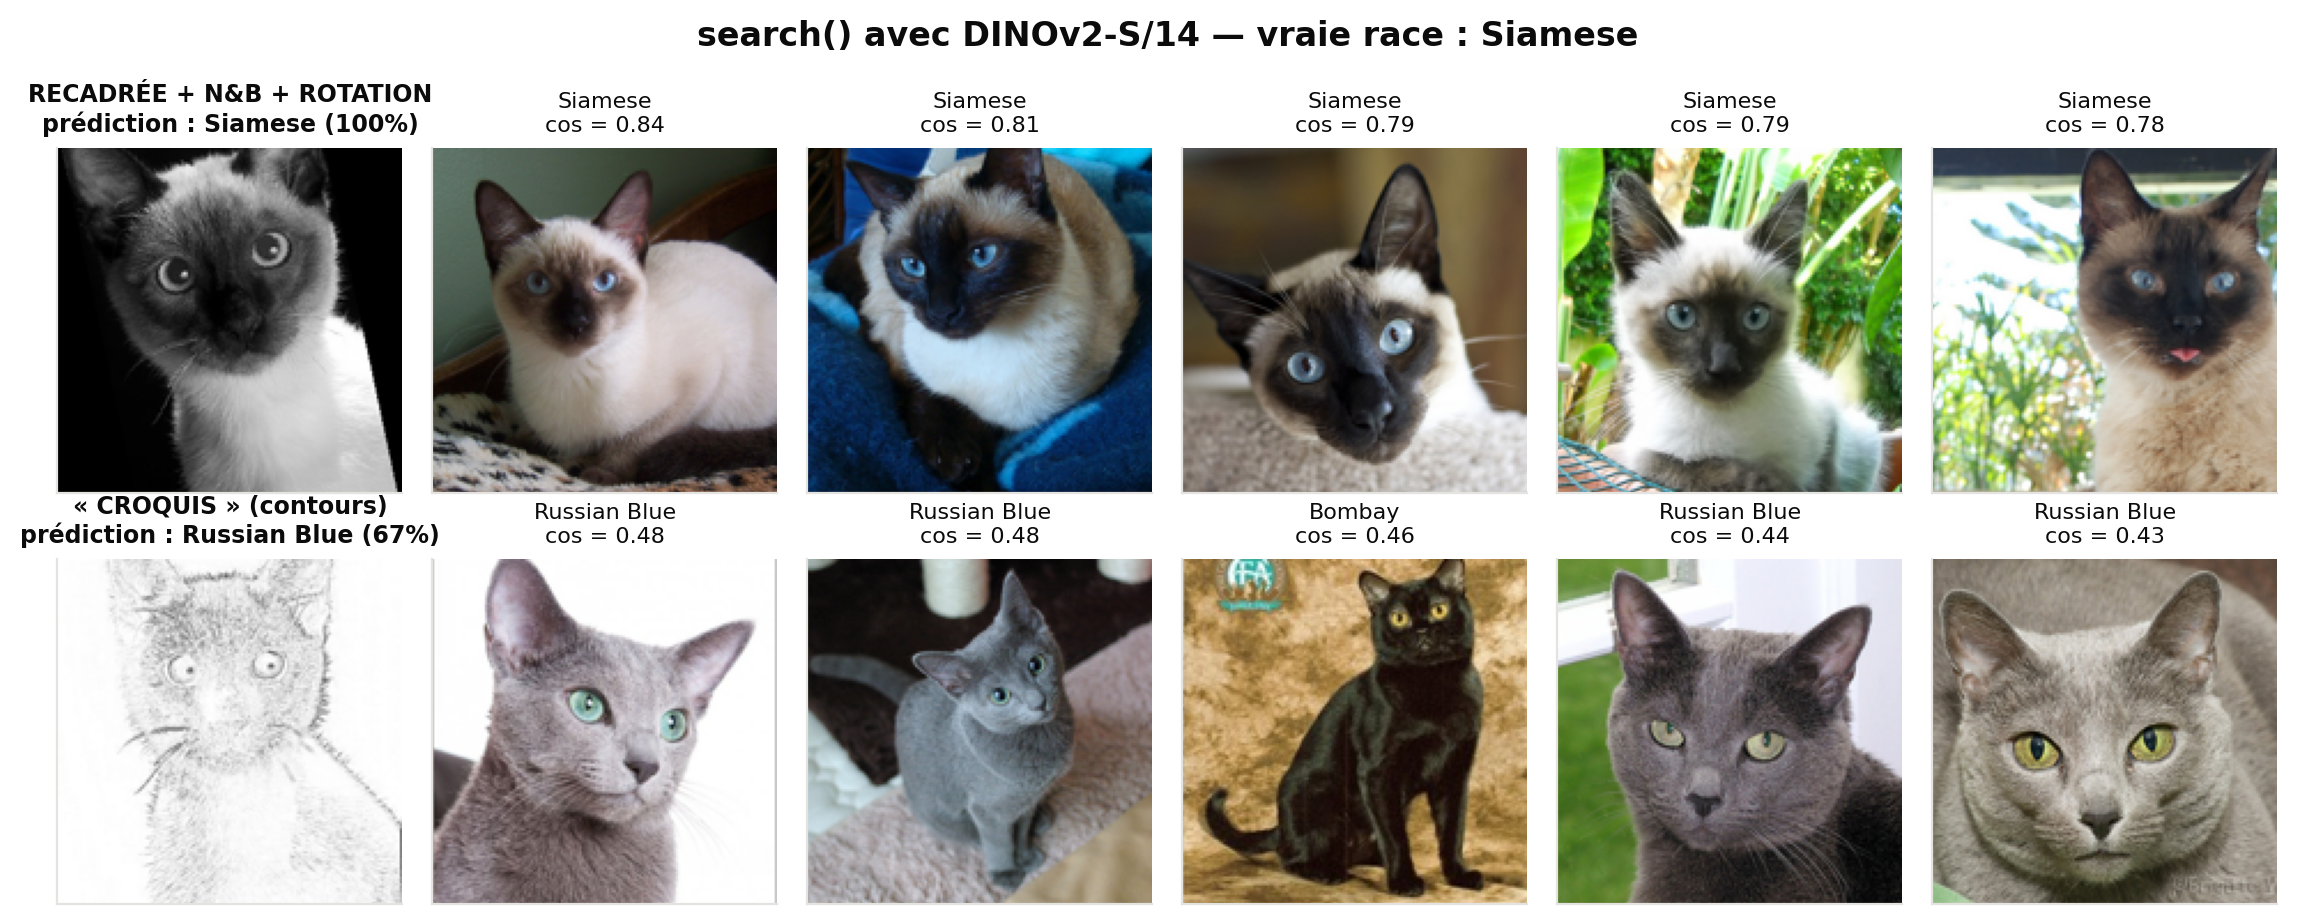
\includegraphics[width=0.94\linewidth,height=0.7\textheight,keepaspectratio]{fig_search_demo.png}\\[1mm]
  \footnotesize Requêtes \textbf{absentes de la galerie} (vraie race : \RsearchTrue)\\
  \ok{} recadrée + N\&B + rotation : \textbf{\RsearchCrop} (\RsearchCropConf{} des votes) \hspace{4mm}
  \ko{} « croquis » : \textbf{\RsearchSketch}, changement de domaine trop fort\\
  {\color{grisE}En direct dans Jupyter : \texttt{search("photo.jpg")} sur vos propres images.}
\end{frame}

\begin{frame}{Résultat 1 : classification sur représentations gelées}
  \begin{columns}[c]
    \begin{column}{0.6\textwidth}
      \centering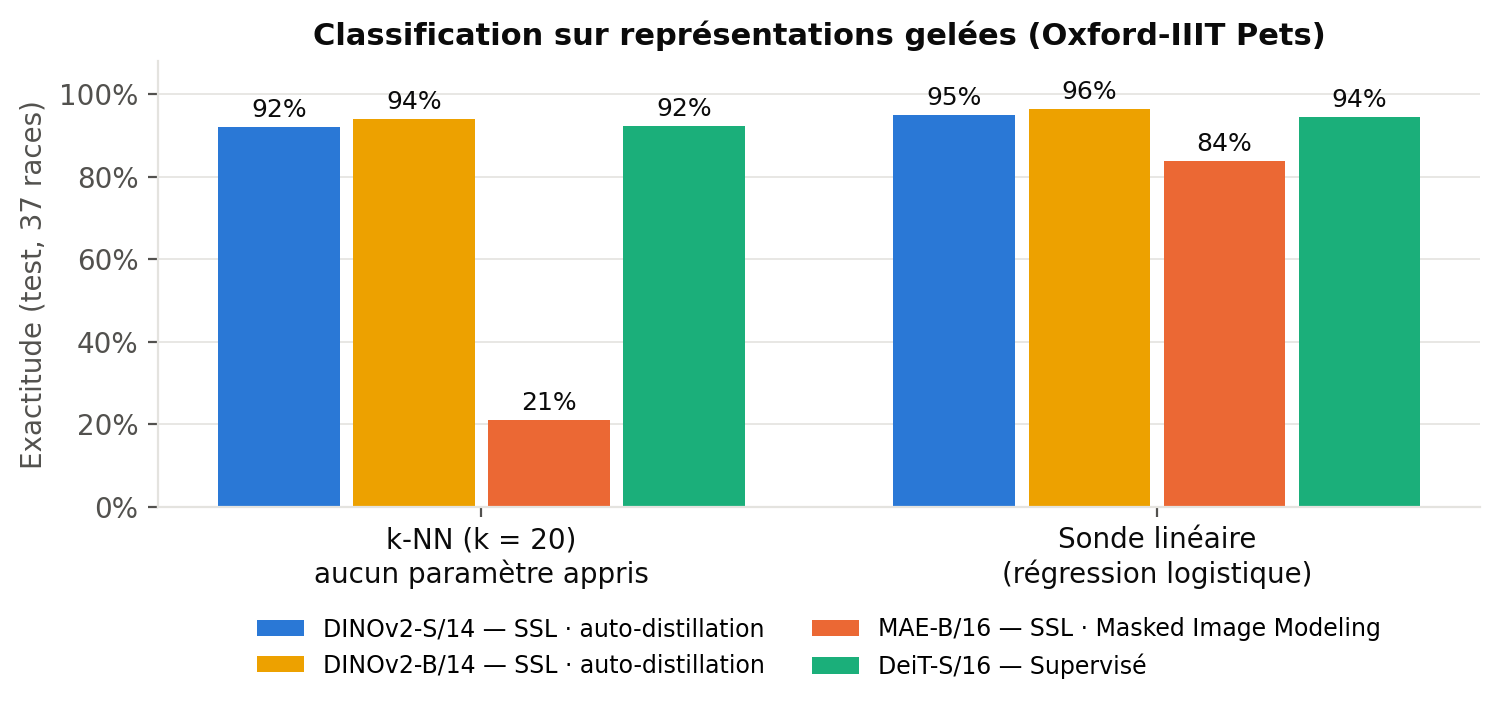
\includegraphics[width=\linewidth]{fig_accuracy.png}
    \end{column}
    \begin{column}{0.38\textwidth}
      \begin{itemize}\small
        \setlength{\itemsep}{1.5mm}
        \item \textbf{DINOv2-B} est le meilleur : \RLinDinoB{} en sonde linéaire, \RKnnDinoB{} avec un simple k-NN (\textbf{0 paramètre appris}).
        \item À taille égale, \textbf{DINOv2-S} (\RLinDinoS) $\approx$ \textbf{DeiT-S supervisé} (\RLinDeit) : même niveau, mais \textbf{sans aucune étiquette}, alors que les labels ImageNet de DeiT couvrent beaucoup de races de Pets.
        \item \textbf{MAE-B} : \RKnnMae{} en k-NN, \RLinMae{} en sonde : features \textbf{non linéaires}, comme prévu par la théorie.
      \end{itemize}
    \end{column}
  \end{columns}
\end{frame}

\begin{frame}{Résultat 2 : recherche d'images similaires}
  \centering
  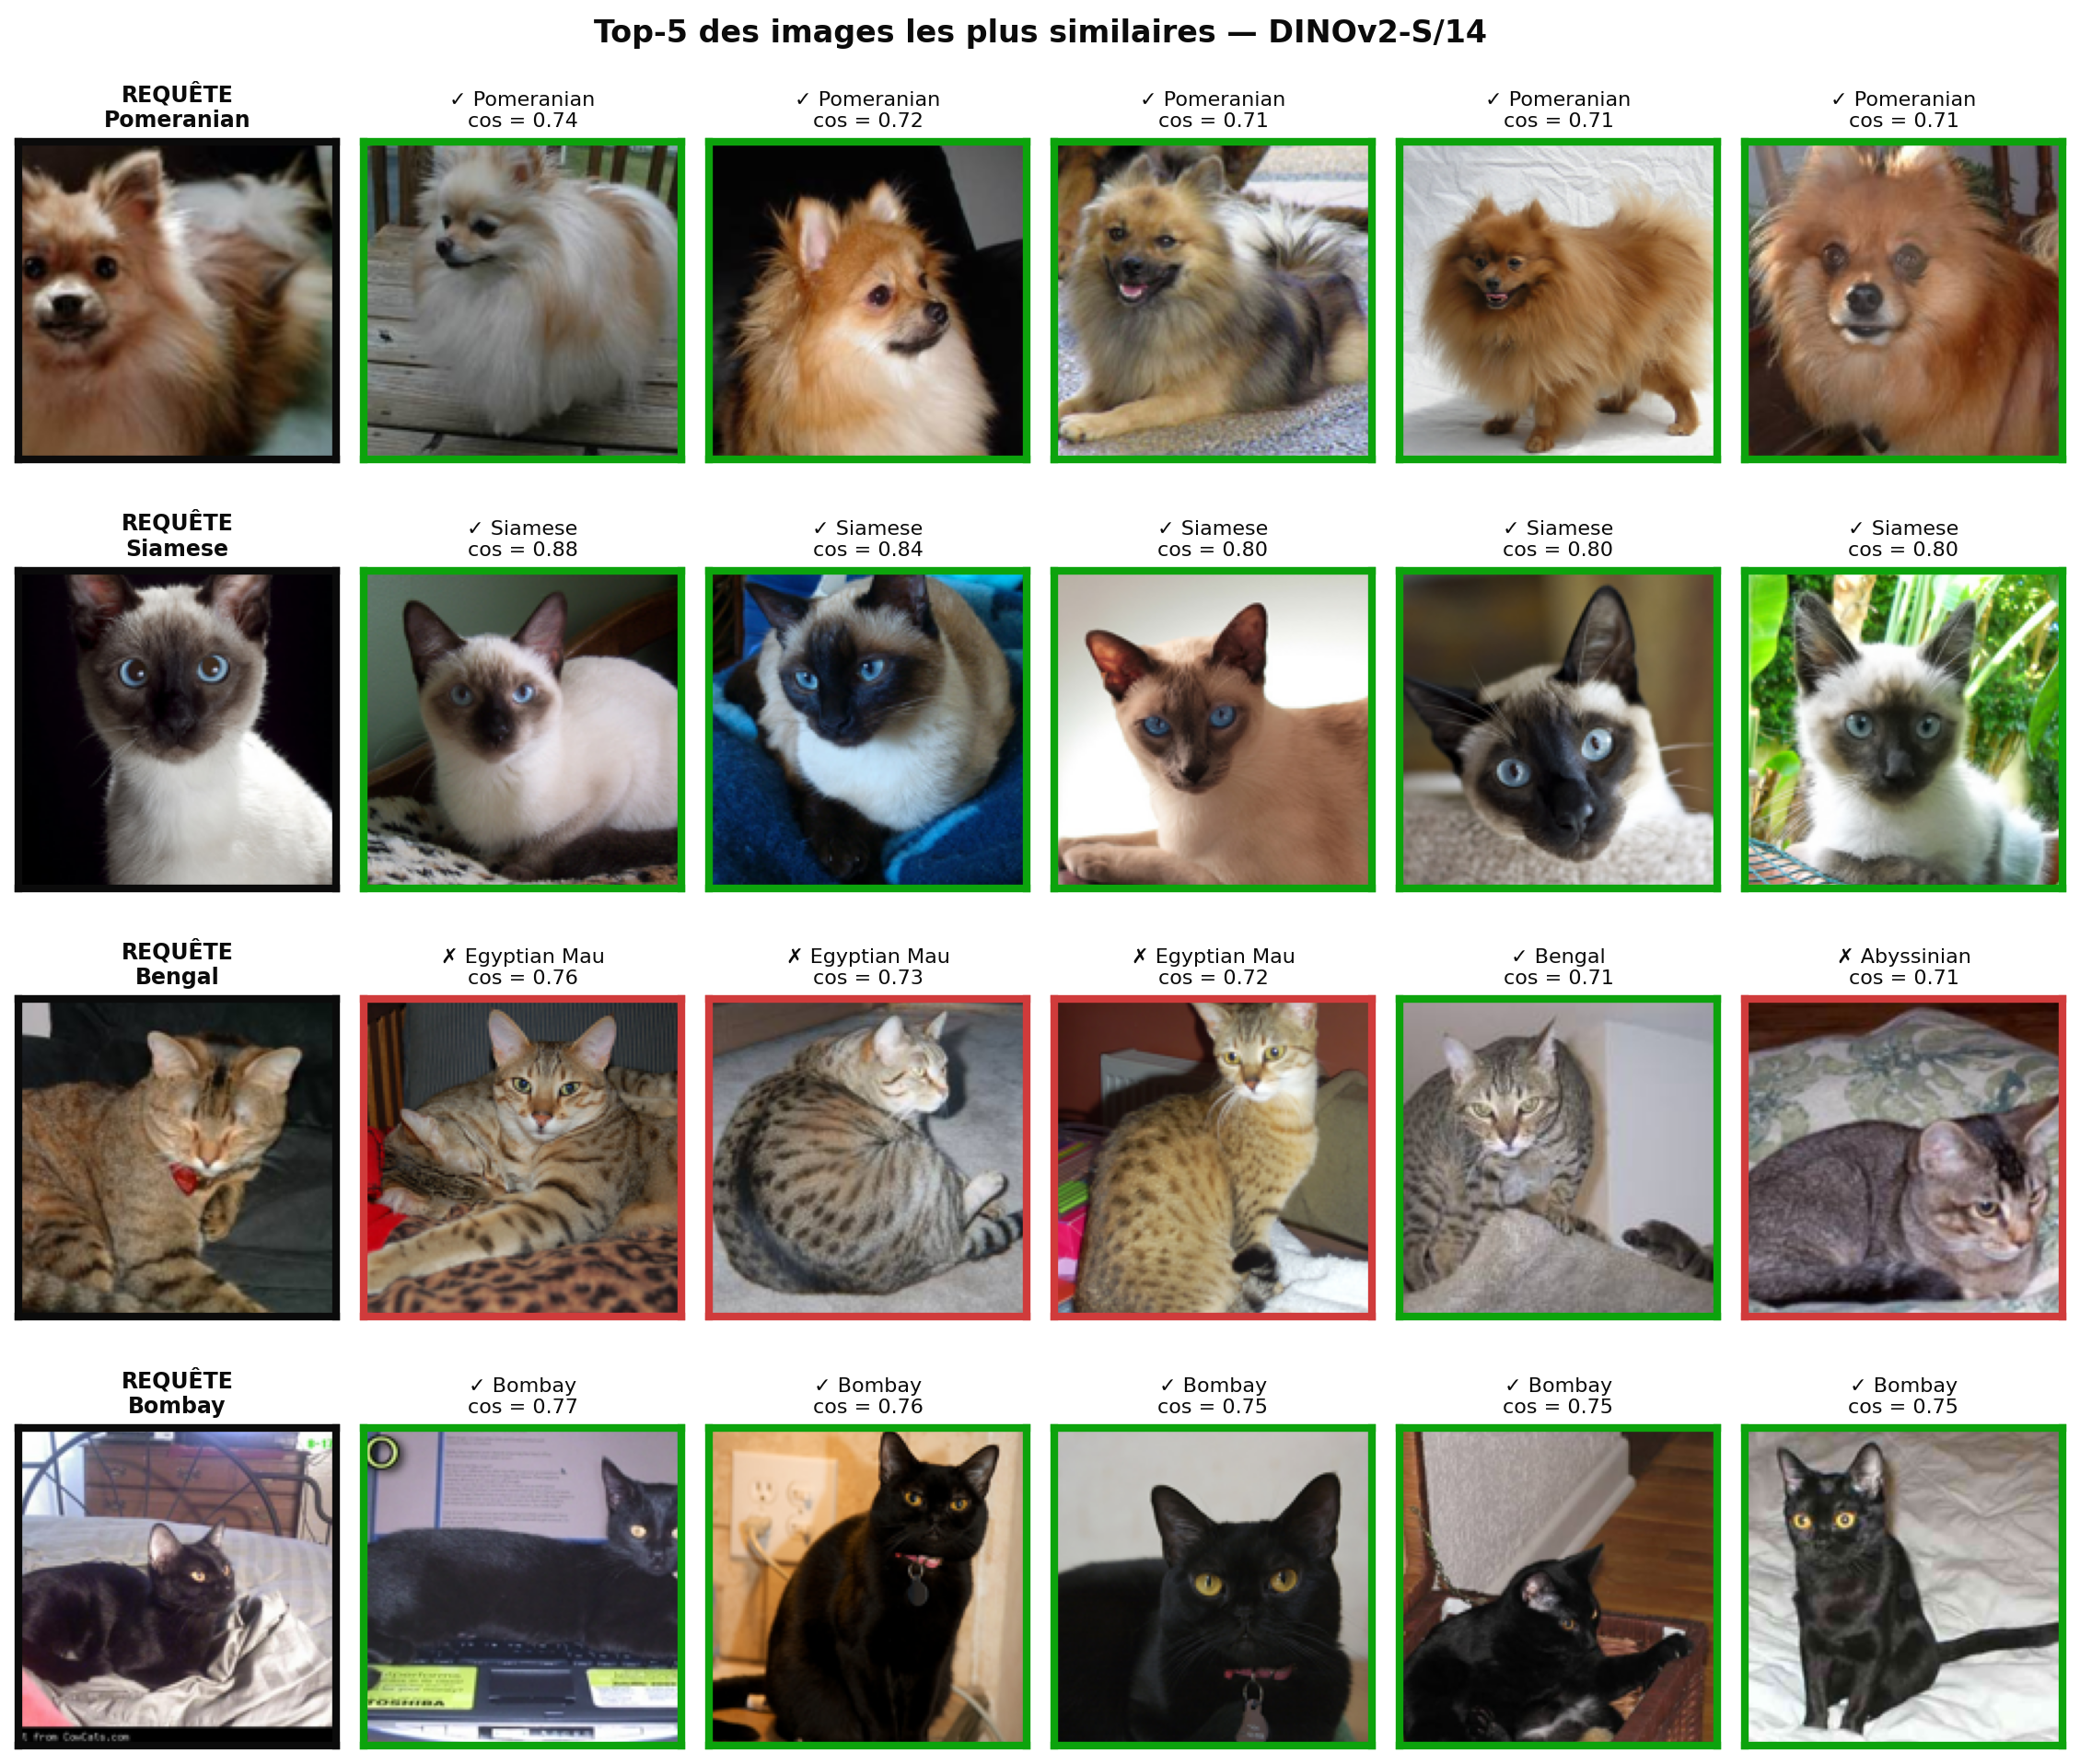
\includegraphics[height=0.66\textheight]{fig_retrieval_dinov2.png}\\[1mm]
  \footnotesize Précision@5 (part des 5 voisins de la même race) : DINOv2-B \textbf{\RPfiveDinoB} $\cdot$ DINOv2-S \RPfiveDinoS{} $\cdot$ DeiT-S \RPfiveDeit{} $\cdot$ MAE-B \RPfiveMae\\
  {\color{grisE}Les erreurs portent sur des races réellement proches (Bengal / Egyptian Mau, Pit Bull / Staffordshire).}
\end{frame}

\begin{frame}{Même requête, quatre encodeurs}
  \begin{columns}[c]
    \begin{column}{0.6\textwidth}
      \centering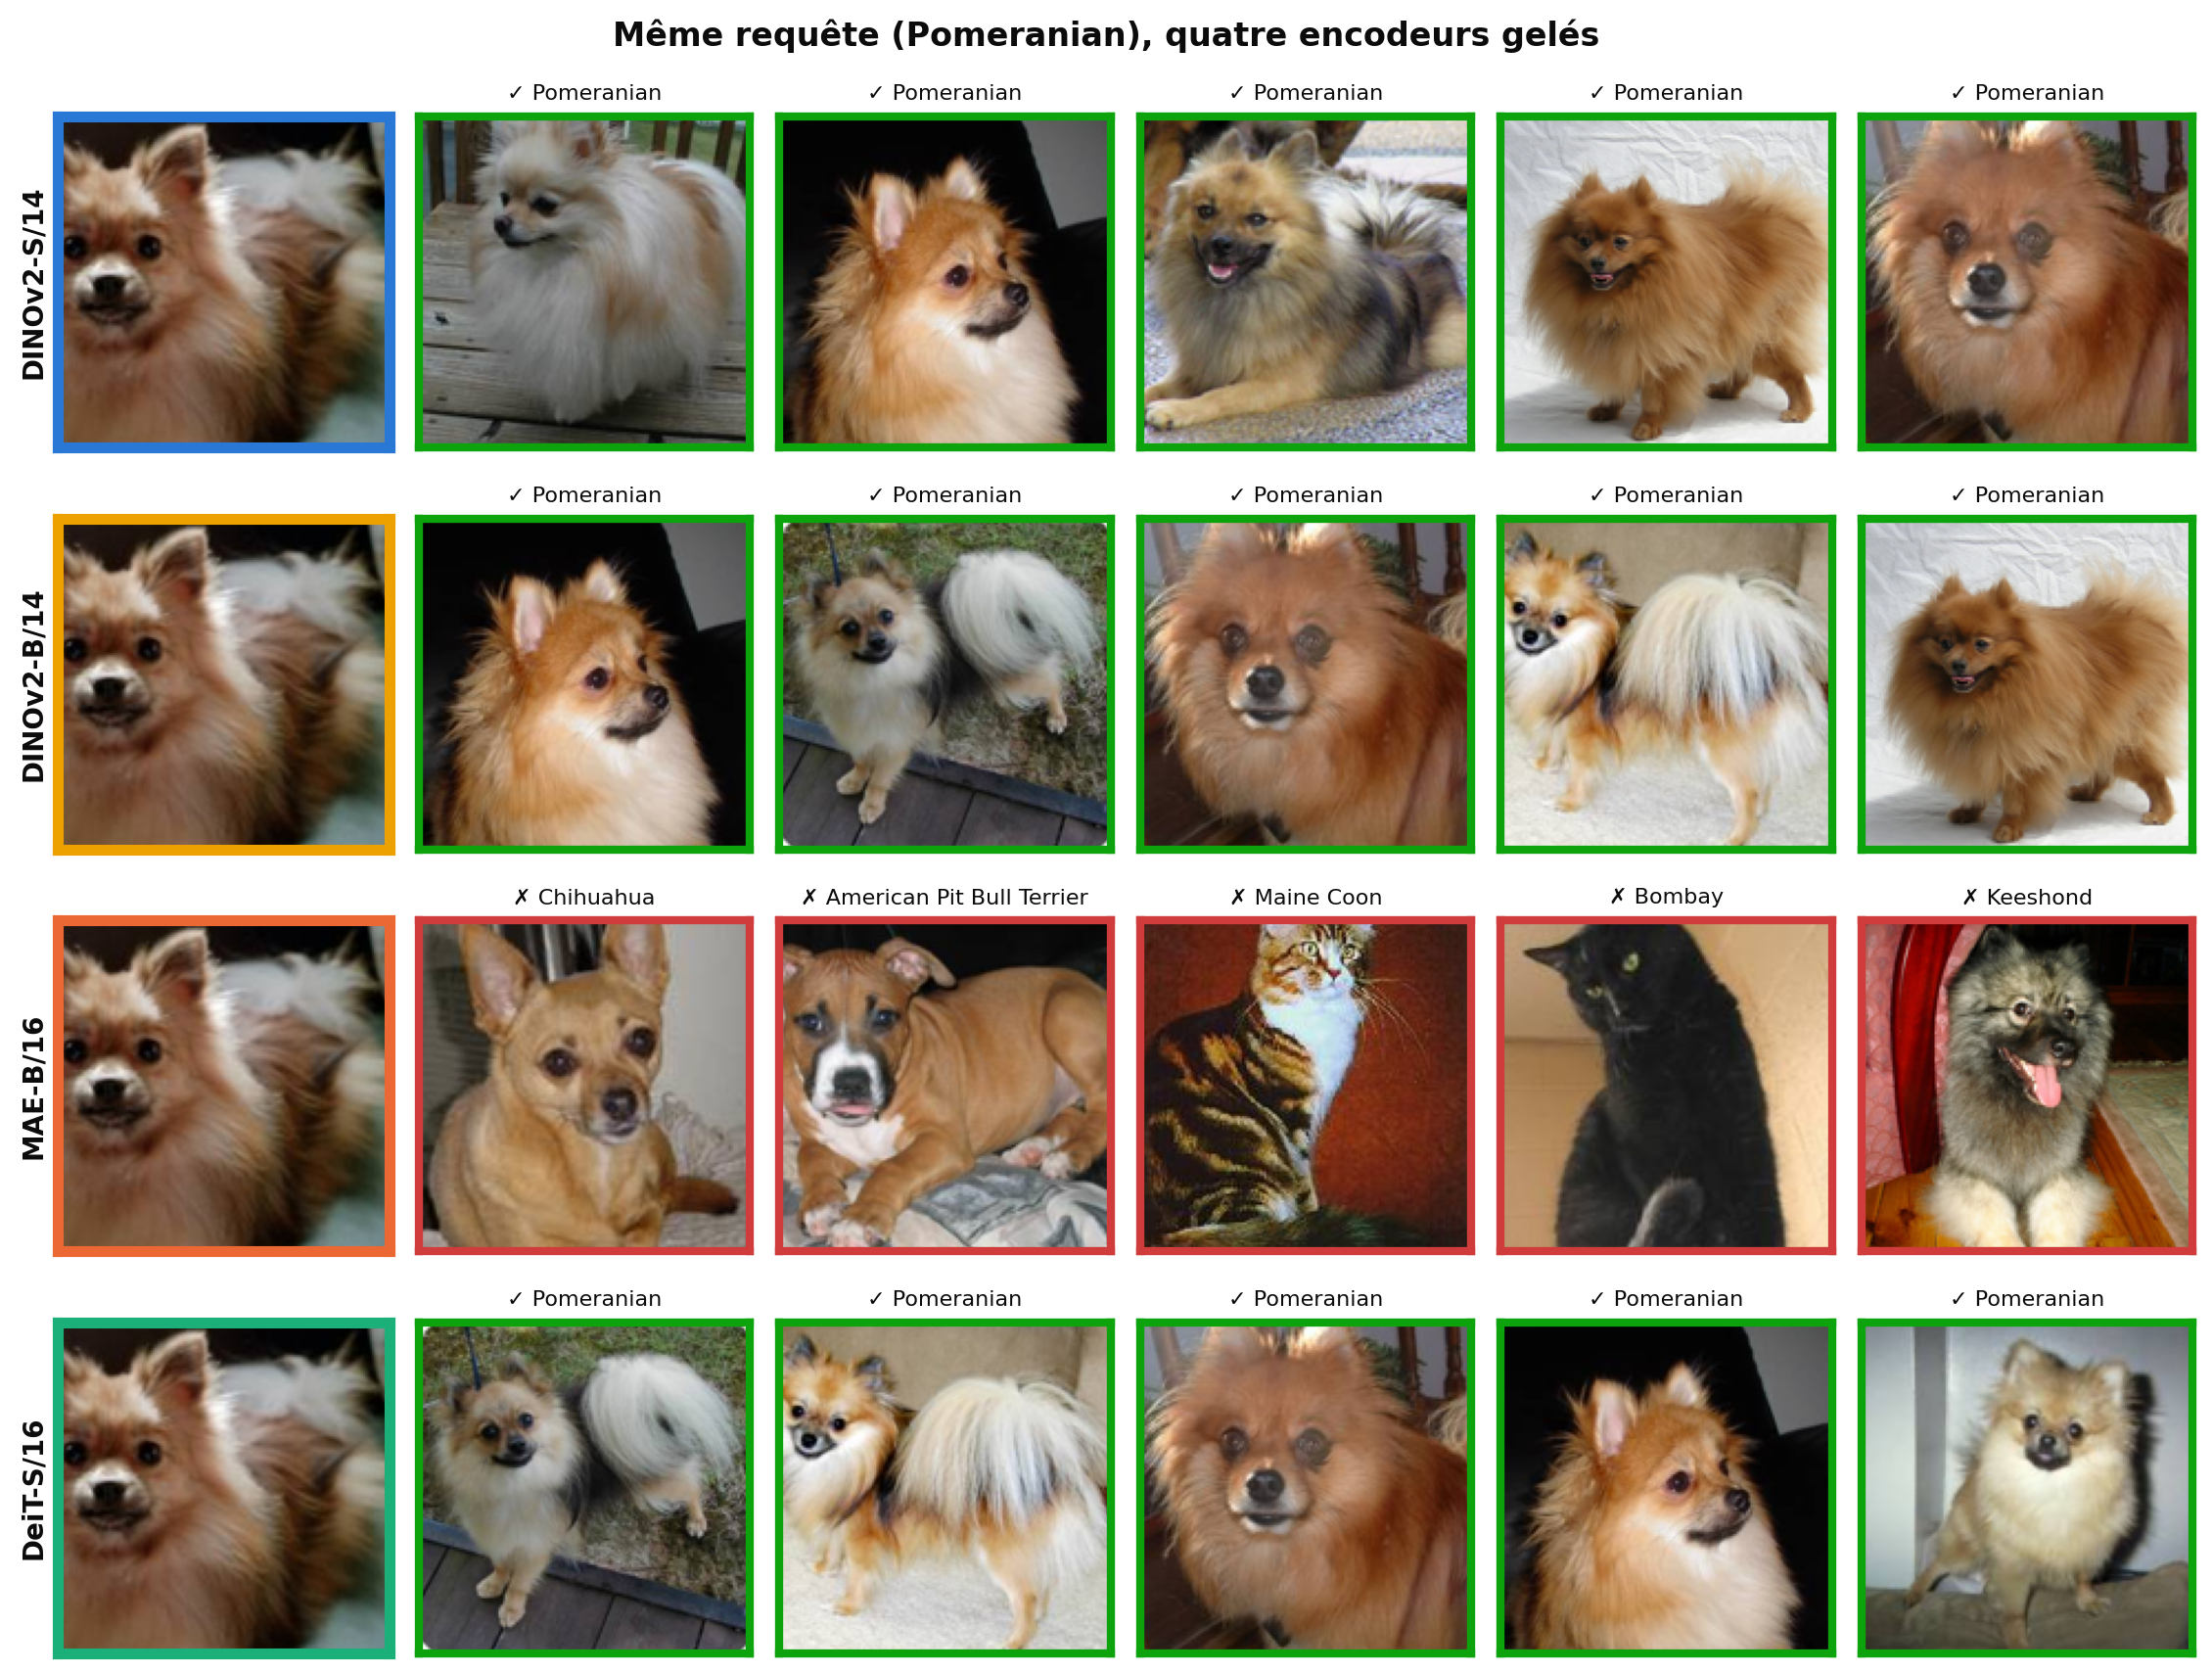
\includegraphics[height=0.8\textheight]{fig_retrieval_compare.png}
    \end{column}
    \begin{column}{0.38\textwidth}
      \small
      \begin{itemize}
        \setlength{\itemsep}{1.5mm}
        \item DINOv2 et DeiT : 5 voisins sur 5 de la \textbf{bonne race}.
        \item MAE : des voisins qui partagent la \textbf{couleur} et la \textbf{pose} (chihuahua fauve, chat sur fond rouge), pas la race.
        \item $\Rightarrow$ MAE encode surtout de l'information de \textbf{bas niveau}, utile après fine-tuning mais pas telle quelle.
      \end{itemize}
    \end{column}
  \end{columns}
\end{frame}

\begin{frame}{Résultat 3 : efficacité en étiquettes}
  \begin{columns}[c]
    \begin{column}{0.6\textwidth}
      \centering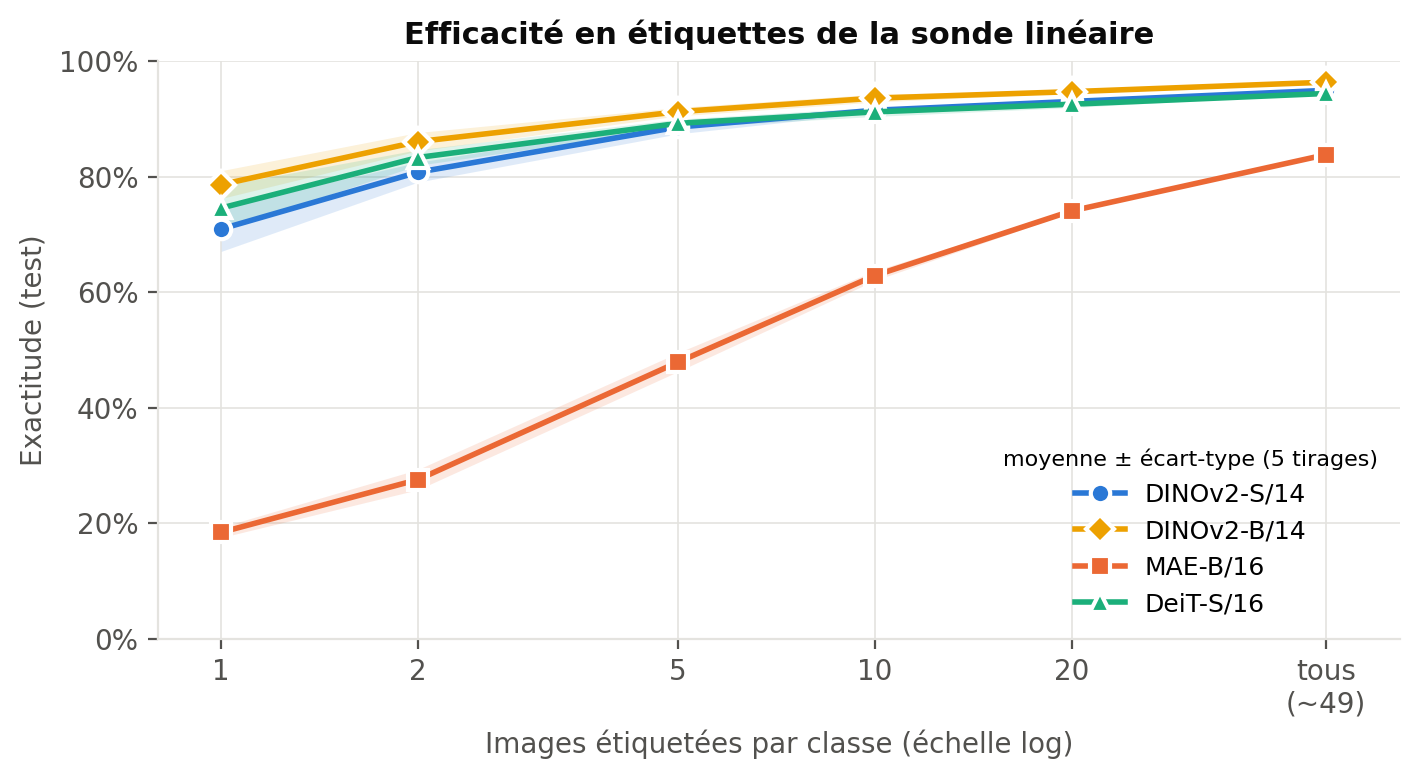
\includegraphics[width=\linewidth]{fig_label_efficiency.png}
    \end{column}
    \begin{column}{0.38\textwidth}
      \footnotesize
      \begin{tabular}{@{}l r r@{}}
        \toprule
        \textbf{Exemples / classe} & \textbf{1} & \textbf{5}\\
        \midrule
        DINOv2-B & \textbf{\RSoneDinoB} & \textbf{\RSfiveDinoB}\\
        DINOv2-S & \RSoneDinoS & \RSfiveDinoS\\
        DeiT-S (supervisé) & \RSoneDeit & \RSfiveDeit\\
        MAE-B & \RSoneMae & \RSfiveMae\\
        \bottomrule
      \end{tabular}
      \vspace{2mm}
      \begin{exampleblock}{Lecture}
        \footnotesize Avec \textbf{une seule} image par classe, DINOv2-B dépasse déjà 75 \% sur 37 races : la connaissance est dans l'encodeur. DeiT-S, supervisé sur des classes proches, reste compétitif ; MAE gelé a besoin de beaucoup plus d'exemples.
      \end{exampleblock}
    \end{column}
  \end{columns}
\end{frame}

\begin{frame}{Résultat 4 : structure de l'espace des représentations}
  \centering
  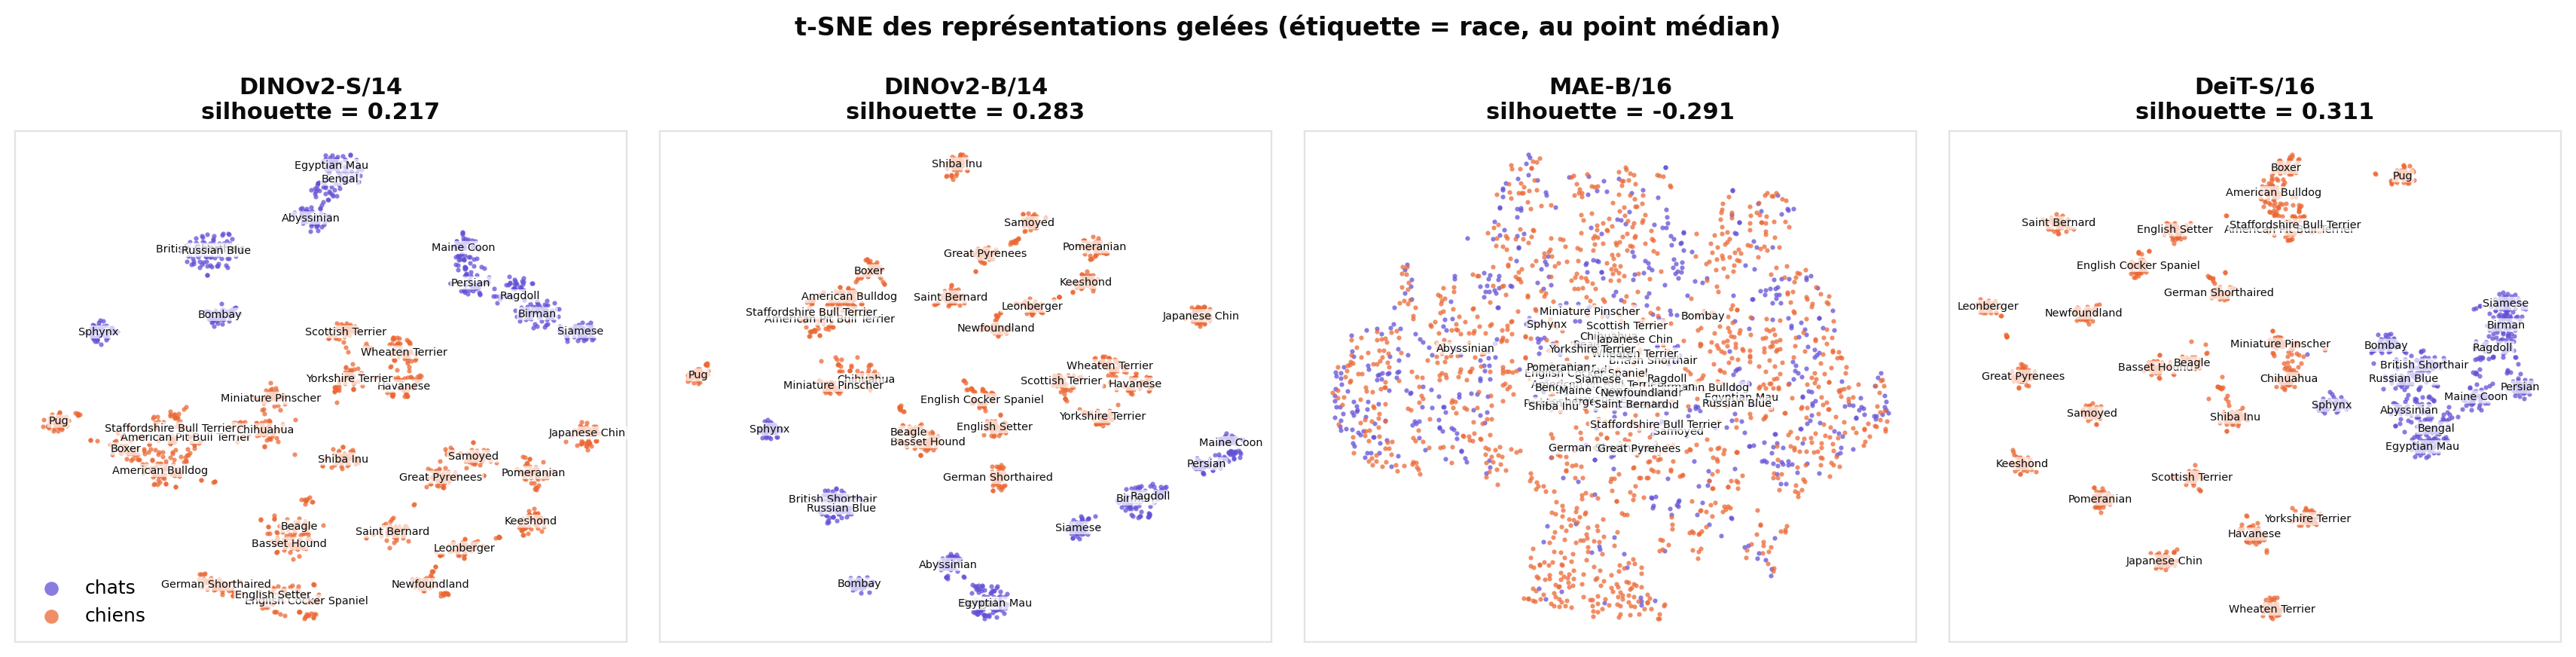
\includegraphics[width=\linewidth,height=0.72\textheight,keepaspectratio]{fig_tsne.png}\\[1mm]
  \footnotesize Silhouette (cosinus, par race ; plus haut = races mieux séparées) : DeiT-S \RSilDeit{} $\cdot$ DINOv2-B \RSilDinoB{} $\cdot$ DINOv2-S \RSilDinoS{} $\cdot$ MAE-B \textbf{\RSilMae}\\
  {\color{grisE}DINOv2 et DeiT regroupent les races (DeiT, entraîné à séparer des classes ImageNet proches, est le plus compact) ; MAE les mélange.}
\end{frame}

\begin{frame}{Résultat 5 : propriété émergente, la segmentation « gratuite »}
  \begin{columns}[c]
    \begin{column}{0.62\textwidth}
      \centering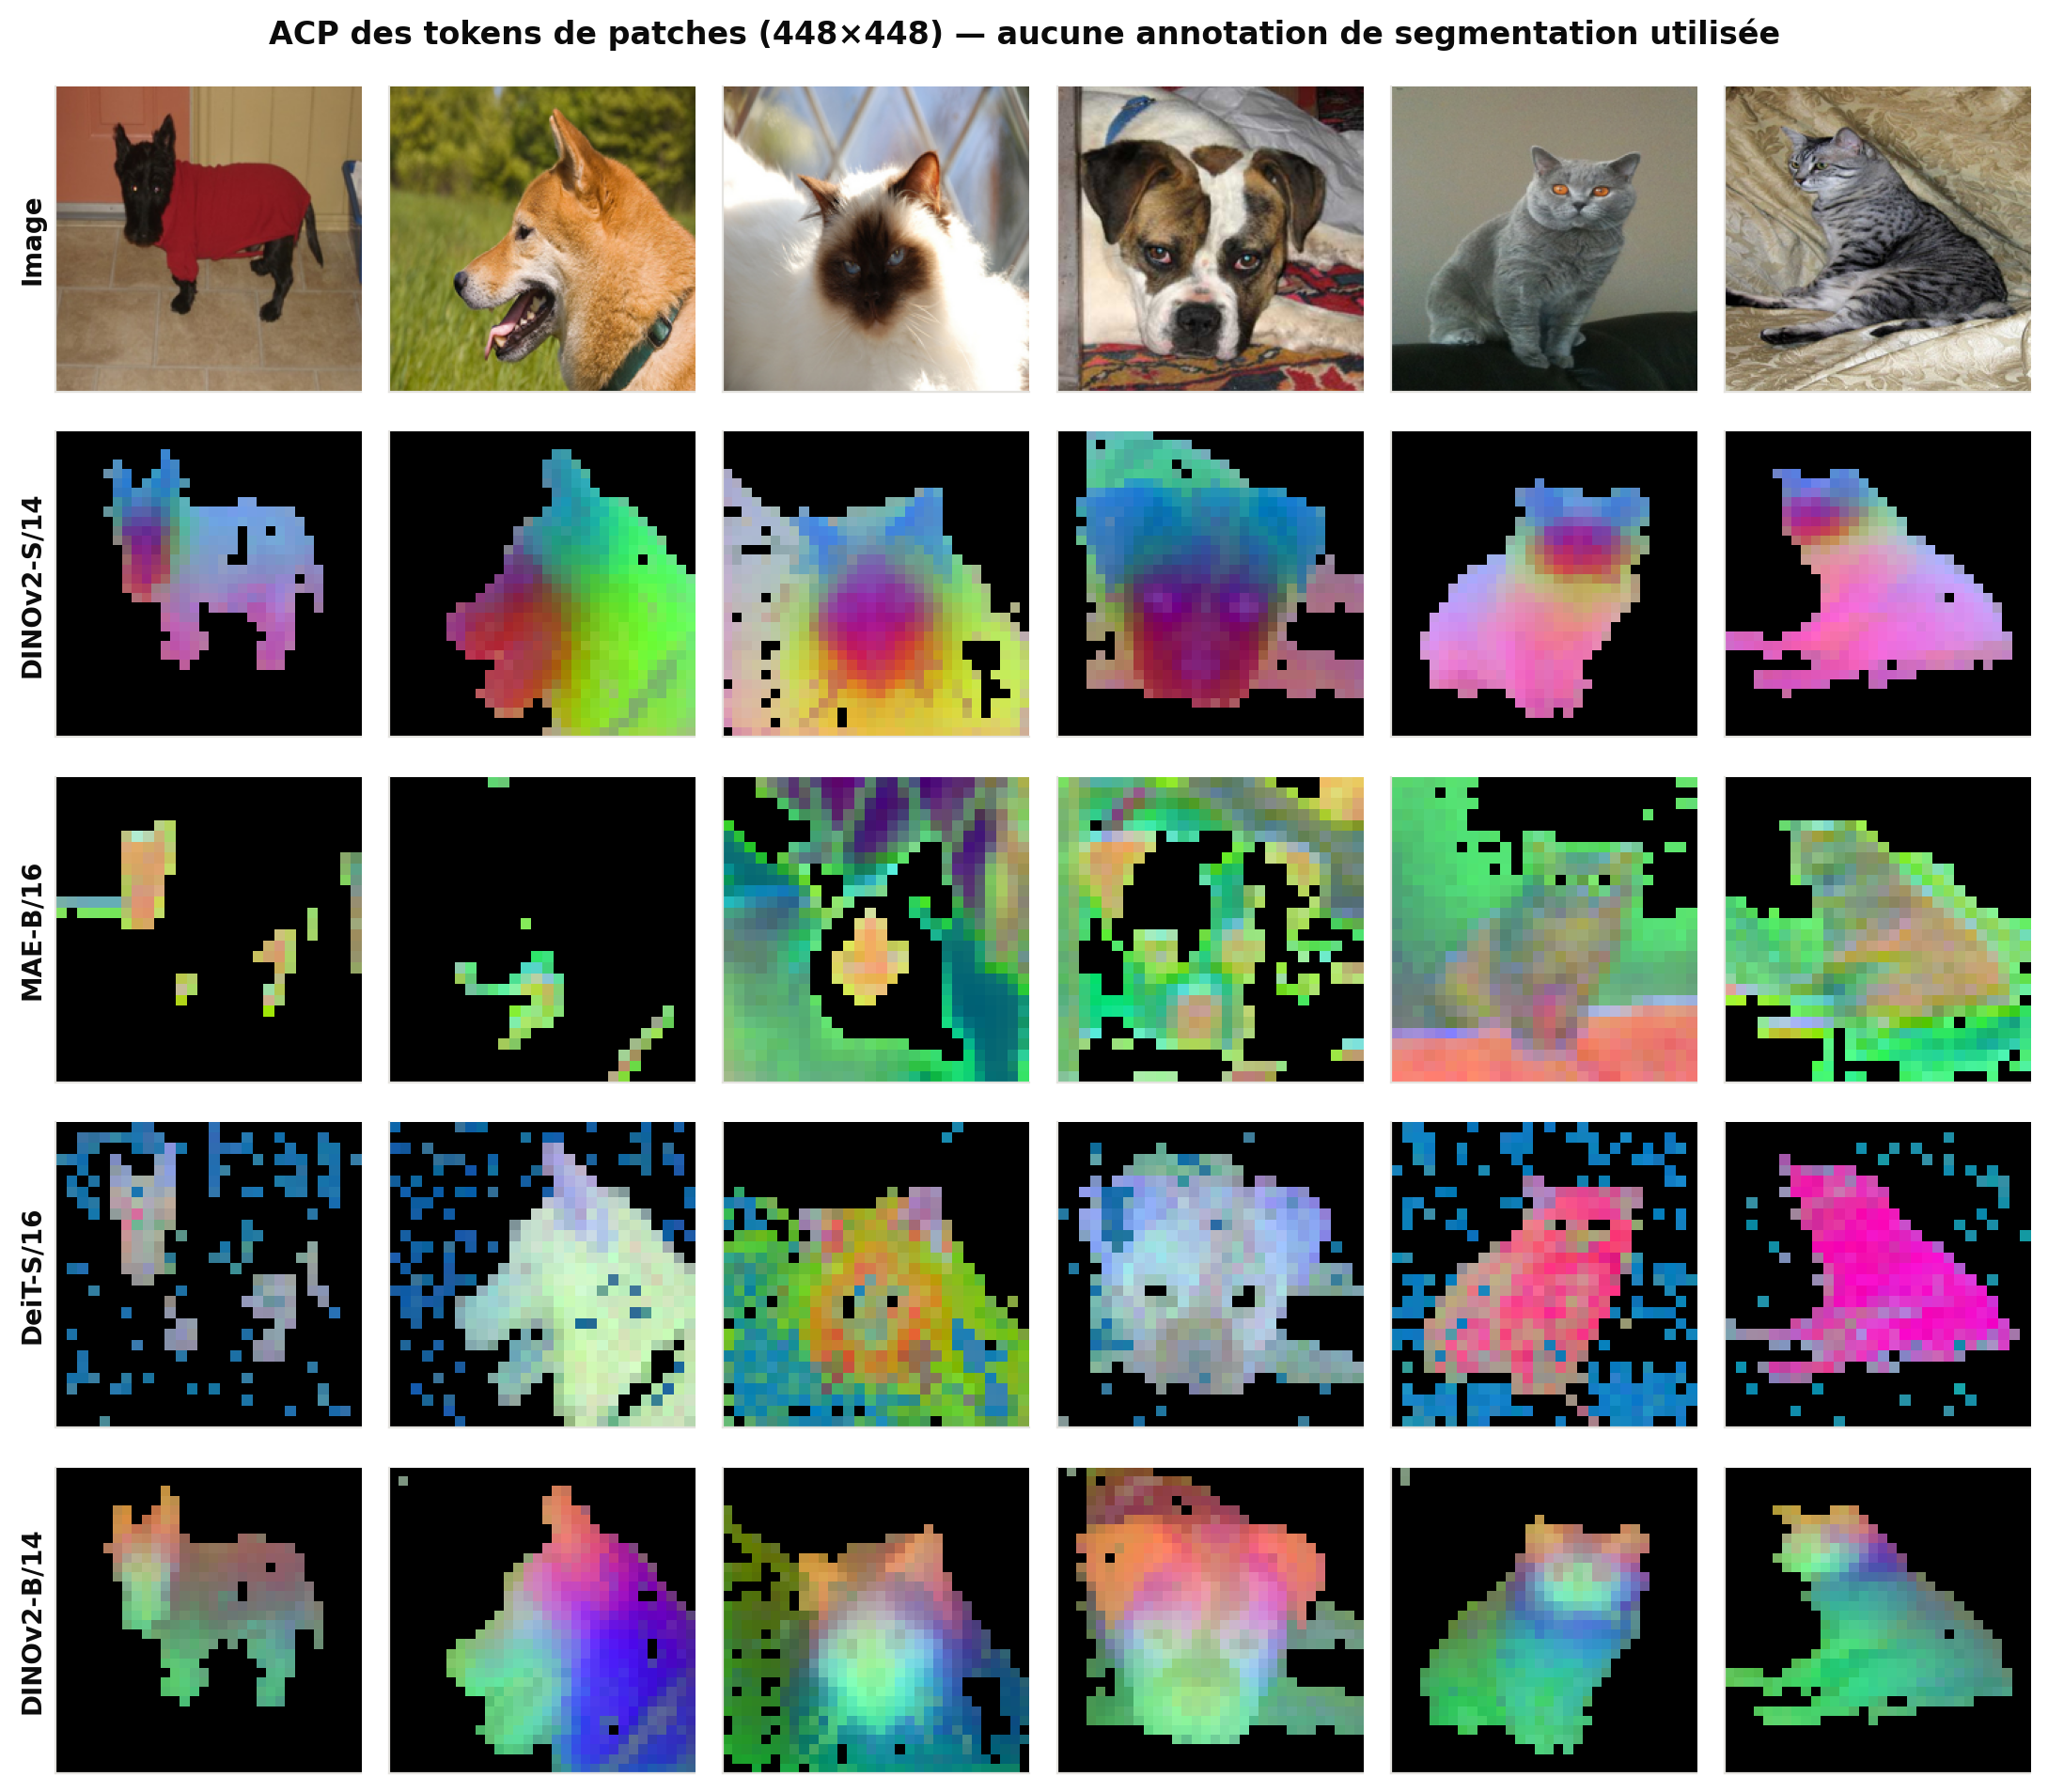
\includegraphics[width=\linewidth,height=0.8\textheight,keepaspectratio]{fig_pca_patches.png}
    \end{column}
    \begin{column}{0.36\textwidth}
      \small ACP des tokens de patches : la 1\textsuperscript{re} composante sépare l'animal du fond, les 3 suivantes (en RVB) révèlent ses \textbf{parties}.\\[2mm]
      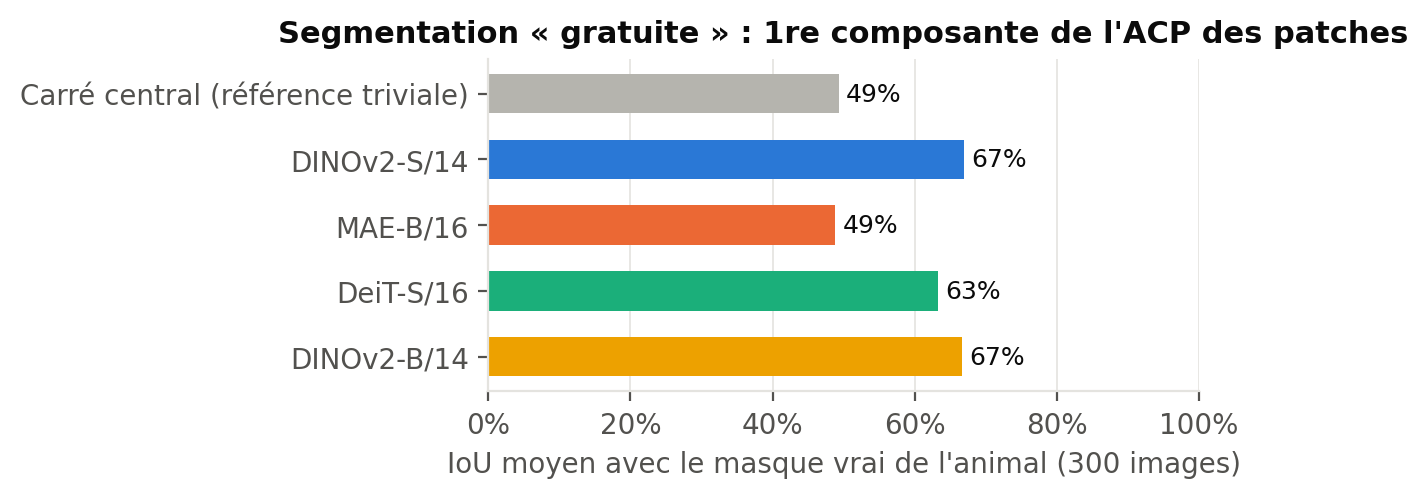
\includegraphics[width=\linewidth]{fig_seg_iou.png}\\
      \footnotesize IoU avec les masques vrais (trimaps), \textbf{sans aucune supervision dense} : DINOv2 \RIouDinoS, DeiT \RIouDeit, MAE \RIouMae{} (= carré central, \RIouCenter).
    \end{column}
  \end{columns}
\end{frame}

\begin{frame}{Coûts de calcul et bilan de l'expérience}
  \begin{columns}[T]
    \begin{column}{0.55\textwidth}
      \footnotesize
      \begin{tabular}{@{}l r r r r@{}}
        \toprule
        \textbf{Encodeur} & \textbf{Params} & \textbf{img/s} & \textbf{VRAM} & \textbf{Linéaire}\\
        \midrule
        DINOv2-S/14 & \RParamsDinoS & \RIpsDinoS & \RVramDinoS & \RLinDinoS\\
        DINOv2-B/14 & \RParamsDinoB & \RIpsDinoB & \RVramDinoB & \textbf{\RLinDinoB}\\
        MAE-B/16 & \RParamsMae & \RIpsMae & \RVramMae & \RLinMae\\
        DeiT-S/16 & \RParamsDeit & \RIpsDeit & \RVramDeit & \RLinDeit\\
        \bottomrule
      \end{tabular}\\[1mm]
      {\scriptsize\color{grisE}Inférence fp16, batch de 32, RTX A2000 4 Go. Extraction de toutes les features : quelques dizaines de secondes par modèle.}
    \end{column}
    \begin{column}{0.42\textwidth}
      \begin{exampleblock}{Ce que montre la démo}
        \footnotesize
        \ok{} DINOv2 gelé : recherche et classification de qualité \textbf{sans fine-tuning} ni étiquette au pré-entraînement\\
        \ok{} DINOv2-B en tête ; DINOv2-S $\approx$ DeiT-S supervisé\\
        \ok{} quelques exemples par classe suffisent\\
        \ok{} segmentation émergente\\
        \ko{} MAE gelé est faible : il faut l'affiner\\
        \ko{} robustesse limitée aux croquis
      \end{exampleblock}
    \end{column}
  \end{columns}
\end{frame}

% ======================================================================
\partie{6}{Comparaison, analyse critique \& conclusion}
% ======================================================================

\begin{frame}{Comparaison des approches}
  \scriptsize
  \begin{tabularx}{\linewidth}{@{}l l c c L L@{}}
    \toprule
    \textbf{Méthode} & \textbf{Signal d'apprentissage} & \textbf{Négatifs} & \textbf{Linéaire IN-1k} & \textbf{Point fort} & \textbf{Limite}\\
    \midrule
    SimCLR & vues augmentées & oui & 69,3 (ResNet-50) & simple & batchs géants\\
    MoCo v3 & vues augmentées & oui & 76,7 (ViT-B) & stable sur ViT & dépend des augmentations\\
    MAE & pixels masqués & non & 68,0 (ViT-B) & rapide, meilleur en fine-tuning & features non linéaires\\
    DINO & vues multi-crop & non & 78,2 (ViT-B/16) & k-NN, attention & hyperparamètres sensibles\\
    \textbf{DINOv2} & DINO + iBOT + KoLeo & non & \textbf{84,5} (ViT-B/14) & features \textbf{gelées} universelles & coût, curation\\
    CLIP & texte associé & oui (texte) & -- & zero-shot (76,2 \% IN) & détails visuels, denses\\
    \bottomrule
  \end{tabularx}
  \vspace{3mm}
  \begin{block}{Lecture}
    \footnotesize Contrastif $\to$ invariances globales ; MIM $\to$ détails locaux mais nécessite un fine-tuning ; \textbf{DINOv2 combine les deux} (image + patches) et l'échelle des données pour obtenir des features directement utilisables.
  \end{block}
  \src{\citet{chen2020simclr,chen2021mocov3,he2022mae,caron2021dino,oquab2024dinov2,radford2021clip}}
\end{frame}

\begin{frame}{Analyse critique}
  \begin{columns}[T]
    \begin{column}{0.32\textwidth}
      \begin{exampleblock}{Performances}
        \footnotesize
        \begin{itemize}
          \item Features gelées au niveau d'un modèle supervisé de même taille, \textbf{sans aucune étiquette} ; meilleures avec plus de paramètres.
          \item Robustes au recadrage et au noir et blanc, moins aux croquis.
          \item Denses : segmentation, profondeur sans tête complexe.
        \end{itemize}
      \end{exampleblock}
    \end{column}
    \begin{column}{0.32\textwidth}
      \begin{alertblock}{Limites}
        \footnotesize
        \begin{itemize}
          \item \textbf{Données} : dépendance à la curation (seeds ImageNet), biais du web.
          \item Pas de lien avec le \textbf{langage} : pas de zero-shot textuel.
          \item Artefacts d'attention (registres), MAE peu séparable.
          \item Évaluation : la sonde linéaire ne mesure pas tout.
        \end{itemize}
      \end{alertblock}
    \end{column}
    \begin{column}{0.32\textwidth}
      \begin{block}{Coûts de calcul}
        \footnotesize
        \begin{itemize}
          \item Pré-entraînement réservé à quelques acteurs (ViT-g : 22\,016 h GPU).
          \item MAE : 3$\times$ moins cher grâce au masquage.
          \item Réutilisation \textbf{très bon marché} : notre démo tourne sur un GPU portable de 4 Go.
        \end{itemize}
      \end{block}
    \end{column}
  \end{columns}
  \vspace{2mm}
  \footnotesize\textbf{Limites de notre expérience} : un seul jeu de données, budgets de pré-entraînement très inégaux entre modèles, recouvrement possible entre races de Pets et classes d'ImageNet.
\end{frame}

\begin{frame}{Conclusion et perspectives}
  \begin{columns}[T]
    \begin{column}{0.5\textwidth}
      \begin{block}{À retenir}
        \small
        \begin{itemize}
          \setlength{\itemsep}{1mm}
          \item Les \textbf{VFM} déplacent l'effort : un pré-entraînement coûteux, puis une adaptation légère.
          \item Le \textbf{SSL} exploite la structure des images : contrastif, masquage, auto-distillation.
          \item \textbf{MAE} : efficace et excellent après fine-tuning.
          \item \textbf{DINOv2} : features \textbf{universelles, gelées}, prêtes pour la recherche, la classification et les tâches denses.
        \end{itemize}
      \end{block}
    \end{column}
    \begin{column}{0.47\textwidth}
      \begin{exampleblock}{Perspectives}
        \small
        \begin{itemize}
          \setlength{\itemsep}{1mm}
          \item \textbf{DINOv3} (2025) : ViT-7B, 1,7 Md d'images, \textit{Gram anchoring} pour préserver les features denses.
          \item Prédiction dans l'espace latent (I-JEPA, V-JEPA pour la vidéo).
          \item Alignement avec le texte (VLM, sujets 6--7) et adaptation par prompts (SAM, sujet 9).
        \end{itemize}
      \end{exampleblock}
    \end{column}
  \end{columns}
  \src{\citet{simeoni2025dinov3,assran2023ijepa,kirillov2023sam}}
\end{frame}

\section{Références}
\begin{frame}[allowframebreaks]{Références}
  \tiny
  \bibliographystyle{abbrvnat}
  \bibliography{../references}
\end{frame}

\begin{frame}[plain,noframenumbering]
  \begin{tikzpicture}[remember picture, overlay]
    \fill[bleuE] (current page.south west) rectangle (current page.north east);
    \fill[orangeE] ($(current page.west)+(0,-0.05)$) rectangle ++(\paperwidth,0.1);
    \node[text=white, font=\Huge\bfseries] at ($(current page.center)+(0,1.0)$) {Merci de votre attention};
    \node[text=white!85!bleuE, font=\Large] at ($(current page.center)+(0,-0.9)$) {Questions \& discussion};
    \node[text=white!70!bleuE, font=\small, align=center] at ($(current page.center)+(0,-2.4)$)
      {NANKOULI M. T. $\cdot$ DIALLO S. $\cdot$ HINIMDOU M. G. $\cdot$ CHAIBOU SAIDOU A. \hspace{4mm}|\hspace{4mm} Encadrant : Pr. ELANSARI};
  \end{tikzpicture}
\end{frame}

\end{document}

% MARC THIERRY NANKOULI